
\documentclass{report}

\usepackage{tlatex}
\usepackage{listings}
\usepackage{xcolor}
\usepackage{comment}
\usepackage{fancyhdr}
\usepackage{amssymb}
\usepackage{inputenc}
\usepackage{svg}

\usepackage{tikz}
\usetikzlibrary{automata, positioning, arrows}


% !TeX spellcheck = en_GB 

% Configure fancyhdr
\pagestyle{fancy}
\fancyhf{} % Clear default header and footer

% Header settings
\fancyhead[L]{\nouppercase{\leftmark}} % Chapter number and title on the left
% \fancyhead[C]{Center Header}    % Centered header
\fancyhead[R]{\thepage}     % Right-aligned header

% Footer settings
% \fancyfoot[L]{Left Footer}      % Left-aligned footer
% \fancyfoot[C]{Page \thepage}    % Centered footer with page number
% \fancyfoot[R]{Right Footer}     % Right-aligned footer

% java -cp /home/richard/dev/tla2tex/tla2tools.jar  tla2tex.TeX  book.tex 

\lstset { %
    language=C++,
    backgroundcolor=\color{black!5}, % set backgroundcolor
    basicstyle=\footnotesize,% basic font setting
}

\title{Learning TLA+ by Examples}
\author{Richard Tang}
\date{\today}
\begin{document}
\maketitle
\tableofcontents

\chapter{Introduction}

\section{Catching Problems Early}

Years ago, I worked on a propietary low power processor in an embedded system.
The processor ran microcode featuring a custom instruction set. To enter a low
power state, a set of (possibly hundreds) instructions were executed. These
instructions progressively puts the system in lower power state. For example:
turn off IP A, then turn off IP B, then turn off the power island to the IPs. To
save cost and power, the low power processor had very limited debuggability
support.\newline

An experienced reader may start to notice some redflags.\newline

If the microcode attempts to access the memory interface when the power island
has been shut off, processor would hang. Since the power island has been shut
off, the physical hardware debug port is also unavailable, leaving the developer
with \textit{no way} of live debugging related problem. At this point the
developer needs to siphon through (possibly hundreds) of instructions to catch
invariant violation \textit{manually}.\newline

As one can imagine, maintaining the microcode was very expensive. Fortunately,
the propietary low power processor only had a handful of instructions, I created
an emulator for this propietary processor to verify the microcode prior to
deploying it on target. The emulator models the processor states as a state
graph, with executed instruction transitions the state machine to the next
state. At every state all the invariants are evaluated to ensure none have been
violated. Some of the invariants included:
\begin{itemize}
    \item Accessing memory interface after power off leads to a hang
    \item Accessing certain register in certain chip revision leads to a hang 
    \item Verify IPs are shut off in the allowed order
\end{itemize}

The verification algorithm was implemented using a \textit{depth-first search}
algorithm, providing \textit{100\%} microcode coverage before deploy on
target.\newline

To generalize, we can model arbitrary system as a set of states with a
collection of invariant that must be upheld at all times. The complexity of the
such arbitrarily system generally grows quadratically as the number of states
grow linearly (eg. in a N state system, adding state N+1 may introduce N
transitions into the new state). There are many engineering problems that
exhibit a large number of states, such as lockless or waitfree data structure,
distributed algorithms, OS scheduler, and more.\newline

\textit{So, how do we build a solution that is correct by design?}

\section{The Generalized Problem}

Fast forward to now: I stumbled across TLA+, a formalized solution of what I was
looking for.\newline

Leslie Lamport invented the TLA+ 1999, but TLA+ didn't appear to have caught on
until the 2010's. My personal opinion is TLA+ was invented ahead of its time,
and the problem complexity finally caught up in the past decade or so to allow
TLA+ to visibly demonstrate its strength.\newline

We are also at a point in the technology curve where vertical scaling is no
longer practical, with CPU speed plateau'd in the past decade or so. The
industry is exploring horizontal scaling solution, such as hardware vendor
focusing adding more CPU cores, or software vendors buying many low end hardware
instead of a few high end hardware. This shifts the technology complexity from
hardware to software, demanding software solution to maximize concurrent
hardware resource utilization. \newline

One slight problem: \textit{The cognitive load of of a person is between 5 to 9
items at most.}\newline

Humans are good at high level reasoning, but not so good at keeping track of
many things happening at the same time. It is hard to enumerate all possible
scenario in one's mind to ensure the design accommodates all the edge cases.
\newline

Consider a distributed system. The system is a cluster of independently
operating entities and need to somehow collectively offer the correct system
behaviour, while any one of the machines may receive instructions out of order,
crash, recover, etc. \newline

Consider a single producer multiple consumer lockless queue. The consumers may 
reserve an index in the queue in certain order, but may release them in different order. 
What if one reader is really slow, and another reader is super fast and possibly 
lapse the slow reader? \newline

Consider an OS scheduler with locks. Assume all the processes have the same
priority. Can a process starve the other processes by repeatedly acquire and
release the lock? How do we ensure scheduling is fair?\newline

The usual \textit{anti-pattern} is to keep bandaiding the design until bugs stop
comming. This is never ideal. Per Murphy's law, anything that can go wrong will
go wrong, and a hard to reproduce bug will come in at the most inconvinient
time. How do we make sure the solution is actually \textit{correct by design}?
To solve this problem, we must rely on tools to do the reasoning \textit{for
us}.

\section{TLA+}

TLA+ is a \textit{system specification language}, with the intent to describe
the system with implementation details removed. TLA+ allows designer to describe
the system as a sequence of states. The designer can expresses transition
condition from one state to another, describe invariants that must hold true in
every state and liveness properties that the overall system should converge to.
The key innovation of TLA+ is once the system is modeled as a finite state
machine, the states can be \textit{exhaustively} explored (via
breath-first-search) to ensure certain properties are held through out the
entire state space (either per state or a sequence of states).\newline

\section{Target Audience}

The intent for the book is to teach reader how to write TLA+ spec for their
design to provide confidence in \textit{design correctness}. The content to this
book is appropriate for software designer, hardware designer, system architect,
and such.\newline 

As for the readers: some computing science knowledge is required. One doesn't
need to be expert at a particular language to understand this book; TLA+ is
effectively its own language. This book is example driven and will go through
designs such as lockless queue, simple task scheduler, consensus algorithm, etc.
Reader will likely enjoy a deeper insight if she has some familiarity with these
topics.

\section{Book Layout}

This book was motivated by the intent to solve problems. The book is designed to
be example heavy with many chapter each represnting an problem that can be
modelled using TLA+.\newline

Examples are split into two categories: A set of examples written using native
TLA+ syntax, and another set of examples written using PlusCal (C-like syntax).
I believe they are useful under different use cases. The differences will be
highlighted in their respective sections. All examples will follow a similar 
layout, covering the expected design process (eg. requirement, spec, safety and
liveness properties). \newline

Finally, there will be part that language reference portion that that discuss a
few topics deserving extra attention. The intent is to be using this section of the 
book as a \textit{reference}.

\chapter{TLA+ Primer}

\section{Design Intent}

The key insight into TLA+ is modelling a system as a state machine. A simple
digital clock can be represented by two variables, hour and minute and the
number of possible states in a digital clock is $24 * 60 = 1440$.  For example,
10:01 is the next state 10:00 can transition to.  Extrapolating further, Asssume
an arbitrarily system described by N variables, each variable having K possible
values such arbitrary system can have up to $N^K$ state.\newline

For every specification, designer can specify \textit{safety} proerty (or
invariants) that must be true in \textit{every} states. For example, in any
state of the digital clock hour \textit{must} be between 0 to 23, or formally
described as $hour \in 0..23$. Similarly, $minute \in 0..59$. More generic
invariant examples include: in any state, only one thread has exclusive access
to a critical region, all variables in the system are within allowable value,
the resource allocation manager never allocates more than available resources,
etc. \newline

Designer can also specify \textit{liveness} property. These are properties that
are satisfied by a \textit{sequence of state}. One liveness property for the
digital clock could be when the clock is $10:00$, it will eventually become
$11:00$ (\textit{$10:00$ leads to $11:00$}). More generic liveness property
include: a distributed system eventually converges, the scheduler eventually
schedules every tasks in the task queue, the resource allocation manager fairly
allocates resources, etc. \newline

TLC checks a TLA+ spec using \textit{breath-first search} algorithm to explore
\textit{all} states in the state machine and ensure safety and liveness
properties are upheld. TLA+ specifies the system using \textit{propositional
logic}. 

\section{Requirement}

In this example, we will specify a \textit{digital clock}. The digital clock has
a few simple requirements:
\begin{itemize}
    \item Two variables to represent state: hour and minute
    \item The clock increment one minute at a time
    \item The clock wraps around at midnight (ie. 23:59 transitions to 00:00)
\end{itemize}

\section{Spec}

The \textit{Init} state of such system can be described as: \newline
\begin{tla}
    Init ==
        /\ hour = 0
        /\ minute = 0
\end{tla}
\begin{tlatex}
\@x{\@s{16.4} Init \.{\defeq}}%
\@x{\@s{32.8} \.{\land} hour \.{=} 0}%
\@x{\@s{32.8} \.{\land} minute \.{=} 0}%
\end{tlatex}
 \newline

$\defeq$ is the \textit{defines equal} symbol and $\land$ is the \textit{logical
and} symbol. The above TLA+ syntax can be read as \textit{Init} state is defined
as both hour and minute are both 0.\newline

The spec also always include a $Next$ definition, an \textit{action formula}
describing how the system transition from one state to another. Action formula
contains \textit{primed} variables what happens to the variable in its next
state. The $Next$ action for the digital clock can be defined as:\newline

\begin{tla}
    NextHour ==
        /\ minute = 59 
        /\ hour' = (hour + 1) % 24
        /\ minute' = 0
    NextMinute == 
        /\ minute # 59
        /\ hour' = hour 
        /\ minute' = minute + 1 
    Next ==
        \/ NextMinute
        \/ NextHour
\end{tla}
\begin{tlatex}
\@x{\@s{16.4} NextHour \.{\defeq}}%
\@x{\@s{32.8} \.{\land} minute \.{=} 59}%
\@x{\@s{32.8} \.{\land} hour \.{'} \.{=} ( hour \.{+} 1 ) \.{\%} 24}%
\@x{\@s{32.8} \.{\land} minute \.{'} \.{=} 0}%
\@x{\@s{16.4} NextMinute \.{\defeq}}%
\@x{\@s{32.8} \.{\land} minute \.{\neq} 59}%
\@x{\@s{32.8} \.{\land} hour \.{'} \.{=} hour}%
\@x{\@s{32.8} \.{\land} minute \.{'} \.{=} minute \.{+} 1}%
\@x{\@s{16.4} Next \.{\defeq}}%
\@x{\@s{32.8} \.{\lor} NextMinute}%
\@x{\@s{32.8} \.{\lor} NextHour}%
\end{tlatex}
 \newline

Here's a breakdown of what the spec does:
\begin{itemize}
    \item $Next$ can take $NextMinute$ or $NextHour$
    \item $Next$ takes $NextMinute$ when $minute$ is not 59, next hour is hour, next minute is minute + 1. 
    \item $Next$ takes $NextHour$ when $minute$ is 59, next hour is (hour + 1) modulus 24, next minute set to 0
\end{itemize}

Technically it's possible for $Next$ to take both $NextMinute$ and $NextHour$.
This is not possible in this definition as $NextHour$ and $NextMinute$ are
defined in a \textit{mutually exlusively} fashion.\newline

Finally, the spec itself is formally defined as:\newline
\begin{tla}
    vars == <<hour, minute>>
    Spec ==
        /\ Init
        /\ [][Next]_vars
\end{tla}
\begin{tlatex}
\@x{\@s{16.4} vars\@s{0.63} \.{\defeq} {\langle} hour ,\, minute {\rangle}}%
\@x{\@s{16.4} Spec \.{\defeq}}%
\@x{\@s{32.8} \.{\land} Init}%
\@x{\@s{32.8} \.{\land} {\Box} [ Next ]_{ vars}}%
\end{tlatex}
\newline

$\Box[Next]_{vars}$ deserves some special attention:
\begin{itemize}
    \item $vars$ is defined to be \textit{all} variables in the spec. Different
    combination of these variables constitute the states of the system (eg.
    23:59 and 00:00 are both states in the system).
    \item $\Box[Next]_{vars}$ is a \textit{box-action formula}, where
    \textit{Next} is an action and \textit{vars} is a state function.
    \item $\Box$ operator asserts the formula is always true for every step in the behaviour.
    \item And steps in the behaviour is defined as $[Next]_{vars}$, where $Next$
    describe the action and $vars$ capturing all variables representing the state.
\end{itemize}

%  $,  The formula is true iff every
% successive pair of steps in behaviour is a $[Next]_{vars}$. Finally $Spec$ is
% conjunction between $Init$ and $\Box[Next]_{vars}$. Note \textbf{all} TLA+
% specification follows very similar template. There are situation we will need to
% provide \textit{fairness} description - this will be covered later. \newline

\section{Safety}

Safety property describes invariant that must hold true in every state of
system. A common invariant is \textit{type safety} checks. In a digital clock, 
hour can only be in value between 0 to 23, and minute can only be value of 0 to 59:\newline

\begin{tla}
    Type_OK == 
        /\ hour \in 0..23
        /\ minute \in 0..59
\end{tla}
\begin{tlatex}
\@x{\@s{16.4} Type\_OK \.{\defeq}}%
\@x{\@s{32.8} \.{\land} hour \.{\in} 0 \.{\dotdot} 23}%
\@x{\@s{32.8} \.{\land} minute \.{\in} 0 \.{\dotdot} 59}%
\end{tlatex}

\section{Liveness}

Liveness property verifies certain behavioural across a sequence of state. One
liveness property can be confirming the clock wraps around correctly at
midnight (which involves mutliple states): \newline

\begin{tla}
    Liveness ==
        /\ hour = 23 /\ minute = 59 ~> hour = 0 /\ minute = 0
\end{tla}
\begin{tlatex}
\@x{\@s{16.4} Liveness \.{\defeq}}%
 \@x{\@s{32.8} \.{\land} hour \.{=} 23 \.{\land} minute \.{=} 59 \.{\leadsto}
 hour \.{=} 0 \.{\land} minute \.{=} 0}%
\end{tlatex}
\newline

$\leadsto$ is the \textit{leads to} operator, suggesting something is eventually
true. TLA+ provides a set of formulas that can be used to describe liveness
property.\newline 

To verify liveness, we need to modify the spec slightly to enable
\textit{fairness} to prevent \textit{stuttering}. In plain terms, fairness
ensure \textit{something} always happen in every step, allowing the states to
transition. Without fairness the spec is allowed to \textit{do nothing} as next
step, this means liveness condition may fail because the spec permits the system
to do nothing in perpetuity as next state. Fairness will be covered in more
detailed in later chapter.\newline

\begin{tla}
    Spec ==
        /\ Init
        /\ [][Next]_vars
        /\ WF_vars(Next)
\end{tla}
\begin{tlatex}
\@x{\@s{16.4} Spec \.{\defeq}}%
\@x{\@s{32.8} \.{\land} Init}%
\@x{\@s{32.8} \.{\land} {\Box} [ Next ]_{ vars}}%
\@x{\@s{32.8} \.{\land} {\WF}_{ vars} ( Next )}%
\end{tlatex}
\newline

$WF_{vars}(Next)$ is the fairness qualifier.

% TODO: insert reference here to specifying systems 8.1 

\section{Model Checker}

The TLA+ spec can be verified using TLC model checker. The TLC model checker
runs the spec and verifies all configured safety and liveness properties are
satisfied during execution. To run TLC, we need two things:
\begin{itemize}
    \item clock.tla - the spec itself
    \item clock.cfg - the corresponding configuration file
\end{itemize}

For reference, clock.tla spec is listed below:

\begin{tla}
--------------------------- MODULE clock ----------------------------
EXTENDS Naturals
VARIABLES hour, minute
vars == <<hour, minute>>
Type_OK == 
    /\ hour \in 0..23
    /\ minute \in 0..59
Liveness ==
    /\ hour = 23 /\ minute = 59 ~> hour = 0 /\ minute = 0
Init ==
    /\ hour = 0
    /\ minute = 0
NextMinute ==
    /\ minute = 59 
    /\ hour' = (hour + 1) % 24
    /\ minute' = 0
NextHour == 
    /\ minute # 59
    /\ hour' = hour 
    /\ minute' = minute + 1 
Next ==
    \/ NextMinute
    \/ NextHour
Spec ==
  /\ Init
  /\ [][Next]_vars
  /\ WF_vars(Next)
=============================================================================
\end{tla}
\begin{tlatex}
\@x{}\moduleLeftDash\@xx{ {\MODULE} clock}\moduleRightDash\@xx{}%
\@x{ {\EXTENDS} Naturals}%
\@x{ {\VARIABLES} hour ,\, minute}%
\@x{ vars \.{\defeq} {\langle} hour ,\, minute {\rangle}}%
\@x{ Type\_OK \.{\defeq}}%
\@x{\@s{16.4} \.{\land} hour \.{\in} 0 \.{\dotdot} 23}%
\@x{\@s{16.4} \.{\land} minute \.{\in} 0 \.{\dotdot} 59}%
\@x{ Liveness \.{\defeq}}%
 \@x{\@s{16.4} \.{\land} hour \.{=} 23 \.{\land} minute \.{=} 59 \.{\leadsto}
 hour \.{=} 0 \.{\land} minute \.{=} 0}%
\@x{ Init \.{\defeq}}%
\@x{\@s{16.4} \.{\land} hour \.{=} 0}%
\@x{\@s{16.4} \.{\land} minute \.{=} 0}%
\@x{ NextMinute \.{\defeq}}%
\@x{\@s{16.4} \.{\land} minute \.{=} 59}%
\@x{\@s{16.4} \.{\land} hour \.{'} \.{=} ( hour \.{+} 1 ) \.{\%} 24}%
\@x{\@s{16.4} \.{\land} minute \.{'} \.{=} 0}%
\@x{ NextHour \.{\defeq}}%
\@x{\@s{16.4} \.{\land} minute \.{\neq} 59}%
\@x{\@s{16.4} \.{\land} hour \.{'} \.{=} hour}%
\@x{\@s{16.4} \.{\land} minute \.{'} \.{=} minute \.{+} 1}%
\@x{ Next \.{\defeq}}%
\@x{\@s{16.4} \.{\lor} NextMinute}%
\@x{\@s{16.4} \.{\lor} NextHour}%
\@x{ Spec \.{\defeq}}%
\@x{\@s{8.2} \.{\land}\@s{0.16} Init}%
\@x{\@s{8.2} \.{\land}\@s{0.16} {\Box} [ Next ]_{ vars}}%
\@x{\@s{8.2} \.{\land}\@s{0.16} {\WF}_{ vars} ( Next )}%
\@x{}\bottombar\@xx{}%
\end{tlatex}

The corresponding clock.cfg is listed below: 
\begin{lstlisting}
    SPECIFICATION Spec
    INVARIANTS Type_OK
    PROPERTIES Liveness
\end{lstlisting}

Now run TLC and one should see something like this: 
\begin{lstlisting}
Model checking completed. No error has been found.
...
The depth of the complete state graph search is 1440.
\end{lstlisting}

\part{Examples}

\chapter{Blinking LED}

Let's start with a trivial specification of a blinking LED. The intent of this example 
is to demonstrate the core functionalities of TLA+ specification language.

TODO: briefly talk about tla+ and model checker here.

\section{Requirement}

The LED is represented by a boolean variable that can be either 0 or 1.\newline

... that's it.

\section{Spec}

The specification language may appear alienating as it is mathematically
motivated based on propositional logic. Despite the (possibly) daunting syntax,
designer only need to be familiar with a handful of key operators to start
realizing value using TLA+. This chapter will attempt to describe the example in
exhaustive detail to reduce the learning curve.

The following describe the core portion of the blinking LED spec. 

\begin{tla}
--------------------------- MODULE blinking ----------------------------
VARIABLES b 
vars == <<b>>
Init ==
    /\ b = 0
On == 
    /\ b = 0
    /\ b' = 1
Off == 
    /\ b = 1
    /\ b' = 0
Next ==
    \/ Off 
    \/ On
Spec ==
    /\ Init
    /\ [][Next]_vars
========
\end{tla}
\begin{tlatex}
\@x{}\moduleLeftDash\@xx{ {\MODULE} blinking}\moduleRightDash\@xx{}%
\@x{ {\VARIABLES} b}%
\@x{ vars \.{\defeq} {\langle} b {\rangle}}%
\@x{ Init\@s{2.02} \.{\defeq}}%
\@x{\@s{16.4} \.{\land} b \.{=} 0}%
\@x{ On \.{\defeq}}%
\@x{\@s{18.15} \.{\land} b \.{=} 0}%
\@x{\@s{18.15} \.{\land} b \.{'} \.{=} 1}%
\@x{ Off \.{\defeq}}%
\@x{\@s{15.91} \.{\land} b \.{=} 1}%
\@x{\@s{15.91} \.{\land} b \.{'} \.{=} 0}%
\@x{ Next \.{\defeq}}%
\@x{\@s{16.4} \.{\lor} Off}%
\@x{\@s{16.4} \.{\lor} On}%
\@x{ Spec \.{\defeq}}%
\@x{\@s{16.4} \.{\land} Init}%
\@x{\@s{16.4} \.{\land} {\Box} [ Next ]_{ vars}}%
\@x{}\bottombar\@xx{}%
\end{tlatex}

\begin{itemize}
    \item $\defeq$ is the \textit{defines equal} operator 
    \item $\land$ and $\lor$ are the AND and OR operator. The effect
    of these operator follow the natural definition in English: 
    \begin{itemize}
        \item $C \defeq A \land B$: C is true iff A and B are true
        \item $C \defeq A \lor B$: C is true iff A or B is true
    \end{itemize}
    \item The $'$ operator represents the next state. $b'$ represent b's next state. 
    \item $VARIABLES$ keyword defines a list of variables for the spec. In this case 
    the spec defines a variable $b$ which can be either 0 or 1
    \item $vars$ is typically defined as a shorthand to refer to \textit{all}
    variables in the spec. 
\end{itemize}

With the above definition, we can revisit the Action definitions: $Init$ defines
the initial system state, where b is set to 0.\newline 

$Next$ requires more elaboration. TLA+ specifies the system as a collection of
states with transitions between them. In a simplified sense, the state is
described as a collection of ANDs (eg. system is in state C if both A and B are
true), the ORs then describe the states the system can possibly be in (eg.
system can be in state C OR D). Revisiting the example, the blinking LED has two
states:
\begin{itemize}
    \item $On \defeq b = 0 \land b' = 1$: b switches on 
    \item $Off \defeq = 1 \land b' = 0$: b switches off
\end{itemize}

The system's $Next$ state is defined to be one of these states:\newline
$Next \defeq On \lor Off$.\newline

$\Box[Next]_{vars}$ is a \textbf{Box-Action Formula}, where \textit{Next} is an
action and \textit{vars} is a state function. The formula is true iff every
successive pair of steps in behaviour is a $[Next]_{vars}$. Finally $Spec$ is
conjunction between $Init$ and $\Box[Next]_{vars}$. Note \textbf{all} TLA+
specification follows very similar template. There are situation we will need to
provide \textit{fairness} description - this will be covered later. \newline

In short: this specification describes a two-state state machine where b toggles
between 0 and 1.\newline

Note that b can technically be \textit{anything}. b can be 0, 1, -42, a
dinosaur, etc. TLA+ specifies values of $b$ which are valid in the system.

\section{Safety}

The spec so far only defines the possible states - but the \textit{power} of
TLA+ lies in its \textit{properties} description. Safety properties are
invariants that must hold true in \textit{every} state. An invariant in the
blinking LED example is: 
\begin{tla}
    TypeOK == b \in {0, 1}
\end{tla}
\begin{tlatex}
\@x{\@s{16.4} TypeOK \.{\defeq} b \.{\in} \{ 0 ,\, 1 \}}%
\end{tlatex}

This states the only valid value of b is 0 or 1. If b is ever set to anything
else, the spec is invalid.\newline

Some example safety properties include: Only a single thread have exclusive
access to critical section, number of concurrent reads cannot exceed data
available to be read, etc. 

\section{Liveness}

While safety properties describe invariant that must be upheld in every state,
\textit{Liveness} describe properties of a sequence of states. In the blinking
LED example, a liveness property can be the if b is 0, it eventually becomes 1,
and vice versa. This is described below:
\begin{tla}
    Liveness == 
        /\ b = 0 ~> b = 1
        /\ b = 1 ~> b = 0
\end{tla}
\begin{tlatex}
\@x{\@s{16.4} Liveness \.{\defeq}}%
\@x{\@s{32.8} \.{\land} b \.{=} 0 \.{\leadsto} b \.{=} 1}%
\@x{\@s{32.8} \.{\land} b \.{=} 1 \.{\leadsto} b \.{=} 0}%
\end{tlatex}

It is the author's opinion liveness describes the \textit{design essense} behind
the spec. The key characteristic of a system is described by its
\textit{behaviour} across a series of states. Does a distribute algorithm
eventually converge to a working state? Does a resource manager fairly allocate
resources in all scenarios? Does a scheduler ensure all tasks are eventually
scheduled? These are behaviours that are \textit{cannot} be concluded by looking
at a single state, but across a \textit{sequence of state}. Liveness allows 
designer to express and verify these properties.

\section{Model Checking}

Since the blinking LED is trivially specified, the full specification is
included below. For subsequent chapters only snippet will be included. Please
refer to the accompanied material for full spec source. 

TODO: install toolchain 

TODO: commandline

TODO: using TLC

The following is the content of \textit{blinking.tla}:
\begin{tla}
--------------------------- MODULE blinking ----------------------------
EXTENDS Naturals
VARIABLES b 
vars == <<b>>
TypeOK ==
  /\ b \in {0, 1} 
Liveness == 
    /\ b = 0 ~> b = 1
    /\ b = 1 ~> b = 0
Init ==
  /\ b = 0
Next ==
  \/ /\ b = 0
     /\ b' = 1
  \/ /\ b = 1
     /\ b' = 0
Spec ==
  /\ Init
  /\ [][Next]_vars
  /\ WF_vars(Next)
=============================================================================
\end{tla}
\begin{tlatex}
\@x{}\moduleLeftDash\@xx{ {\MODULE} blinking}\moduleRightDash\@xx{}%
\@x{ {\EXTENDS} Naturals}%
\@x{ {\VARIABLES} b}%
\@x{ vars \.{\defeq} {\langle} b {\rangle}}%
\@x{ TypeOK \.{\defeq}}%
\@x{\@s{8.2} \.{\land} b \.{\in} \{ 0 ,\, 1 \}}%
\@x{ Liveness \.{\defeq}}%
\@x{\@s{16.4} \.{\land} b \.{=} 0 \.{\leadsto} b \.{=} 1}%
\@x{\@s{16.4} \.{\land} b \.{=} 1 \.{\leadsto} b \.{=} 0}%
\@x{ Init \.{\defeq}}%
\@x{\@s{8.2} \.{\land} b \.{=} 0}%
\@x{ Next \.{\defeq}}%
\@x{\@s{8.2} \.{\lor}\@s{1.63} \.{\land} b \.{=} 0}%
\@x{\@s{20.94} \.{\land} b \.{'} \.{=} 1}%
\@x{\@s{8.2} \.{\lor}\@s{1.63} \.{\land} b \.{=} 1}%
\@x{\@s{20.94} \.{\land} b \.{'} \.{=} 0}%
\@x{ Spec \.{\defeq}}%
\@x{\@s{8.2} \.{\land}\@s{0.16} Init}%
\@x{\@s{8.2} \.{\land}\@s{0.16} {\Box} [ Next ]_{ vars}}%
\@x{\@s{8.2} \.{\land}\@s{0.16} {\WF}_{ vars} ( Next )}%
\@x{}\bottombar\@xx{}%
\end{tlatex}

The following is the content of \textit{blinking.cfg}:

\begin{lstlisting}
    SPECIFICATION Spec
    INVARIANTS TypeOK
    PROPERTIES Liveness
\end{lstlisting}

\section{Limitation}

Since TLA+ exhaustively explores all possible state, a linear growth of
variables leads to TLC (temporal logic checker) execution time grows
\textit{exponentially}.This means the specification must be scoped correctly to
limit the state space.\newline

Similarly, if you want to verify concurrent psuedo code implementation in
PlusCal, you can likely at most verify 10s of lines of code.

\chapter{Simple Gossip Protocol}

This section the author's notes on a simple gossip protocol by Andrew Hewler:\newline
https://ahelwer.ca/post/2023-11-01-tla-finite-monotonic/\newline

\section{Requirement}

In a distributed system, a cluster of nodes collectively provide a serivce. A
distributed database may have a collection of 10s to 100s of nodes working
together to offer the service in a geo diverse fashion to be immnue to partial
outage.  The nodes often have requirements to know about each other. In the
context of distributed database, a node may need to know the key range another
of its peers. The cluster needs a way to communicate this information. One such
mechanism is the gossip protocol.\newline

Gossip protocols are used to communicate cluster information in a distributed
fashion, (unsurprisingly) in a distributed system. Without gossip protocol, 
nodes in a cluster learns about its neighbours by contacting a centralized
server. This introduces a single failure point in the system. As the name
suggest, gossip protocol relies on nodes to gossip with each other. The nodes in
the cluster periodically selects a set of neighbors to exchange what it knows
about the cluster. The recency information is part of the gossip message
itself, allowing the node and the peer its talking to quickly decide who has the
latest information on a node, and converge to it. Assume a N node cluster and
each interal a node selects k neighbours to gossip with, the total amount of
gossip propagation time is described logrithmticly below:

\begin{equation} 
    propagation\_time = \log_k N * gossip\_interval
\end{equation}

With the total number of messages exchanged: 
\begin{equation} 
    messages\_exchanged = \log_k N * k
\end{equation}

Now let's look at how a simple gossip protocol can be described by TLA+.

\section{Spec}

In gossip protocol, every node needs to remember all its peers current
version. This can be represented as a two dimension array:\newline
\begin{tla}
    Init == counter = [n \in Node |-> [o \in Node |-> 0]] 
\end{tla}
\begin{tlatex}
 \@x{\@s{16.4} Init \.{\defeq} counter \.{=} [ n \.{\in} Node \.{\mapsto} [ o
 \.{\in} Node \.{\mapsto} 0 ] ]}%
\end{tlatex}
\newline

This defines counter a collection of nodes, where each node also contains a
collection of nodes initialized to 0. The nodes can bump to a new version:\newline
\begin{tla}
    Increment(n) == counter' = [counter EXCEPT ![n][n] = @ + 1]
\end{tla}
\begin{tlatex}
 \@x{\@s{16.4} Increment ( n ) \.{\defeq} counter \.{'} \.{=} [ counter
 {\EXCEPT} {\bang} [ n ] [ n ] \.{=} @ \.{+} 1 ]}%
\end{tlatex}
\newline

Notice increment only bumps node's version. This change needs to be gossiped 
across the cluster:\newline
\begin{tla}
Gossip(n, o) ==                  
    LET Max(a, b) == IF a > b THEN a ELSE b 
    IN counter' = [
        counter EXCEPT ![o] = [
            nn \in Node |->            
                Max(counter[n][nn], counter[o][nn])
            ] 
    ]
\end{tla}
\begin{tlatex}
\@x{ Gossip ( n ,\, o ) \.{\defeq}}%
 \@x{\@s{16.4} \.{\LET} Max ( a ,\, b ) \.{\defeq} {\IF} a \.{>} b \.{\THEN} a
 \.{\ELSE} b}%
\@x{\@s{16.4} \.{\IN} counter \.{'} \.{=} [}%
\@x{\@s{40.89} counter {\EXCEPT} {\bang} [ o ] \.{=} [}%
\@x{\@s{57.29} nn \.{\in} Node \.{\mapsto}}%
\@x{\@s{73.41} Max ( counter [ n ] [ nn ] ,\, counter [ o ] [ nn ] )}%
\@x{\@s{57.29} ]}%
\@x{\@s{16.4} ]}%
\end{tlatex}
\newline

A few things to unpack here:
\begin{itemize}
    \item $n, o$ are the two nodes exchanging gossip. $o$ is the node to be updated
    and $n$ is the neighbor $o$ gossips with.
    \item $LET .. IN$ allows local definition under $LET$ used under
    $IN$. In this case $Max$ is a local macro defined to return maximum between a and b.
    \item $counter'$ (or refered to as counter \textit{prime}) is what the
    variable will be in the next state. TLA+ doesn't provide a way to update a
    variable in a collection, so the convention is to assign a new array to the variable. 
    \item $counter\ EXCEPT ![o] = [...]$ return $counter$ with $counter[o]$
    defined in the bracket. 
    \item where $[...]$ is a collection of nodes with with counter set to the
    max between the current node and neighbour.
\end{itemize}

Finally, the actual spec: \newline
\begin{tla}
    Next == \/ \E n \in Node : Increment(n)
            \/ \E n, o \in Node : Gossip(n, o)
\end{tla}
\begin{tlatex}
 \@x{\@s{16.4} Next \.{\defeq} \.{\lor} \E\, n \.{\in} Node \.{:} Increment (
 n )}%
\@x{\@s{56.23} \.{\lor} \E\, n ,\, o \.{\in} Node \.{:} Gossip ( n ,\, o )}%
\end{tlatex}
\newline

Next supports two possible next steps describe using disjunctions. The first is
bumping the version of a random node, the second is select a pair of nodes to
gossip. Note the \textit{existential qualifier} on both, which basically states
there exists a node n in nodes, or there exists a pair of nodes n, o in nodes,
respectively.\newline

There's a minor problem with the definition above. Gossip protocol, like many
converging protocols, have a \textit{monotonic increasing} requirement. On
failures, the protocol bumps the version, which increases monotonically. Since
TLA+ spec models the system as a graph, a monotonic increasing version number
means the state graph is \textit{infinitely large}. To put the specification back into
finite space, we can normalize the state:\newline

\begin{tla}
GarbageCollect ==
    LET SetMin(s) == CHOOSE e \in s : \A o \in s : e <= o IN
    LET Transpose == SetMin({counter[n][o] : n, o \in Node}) IN
        /\ counter' = [
            n \in Node |-> [
                o \in Node |-> counter[n][o] - Transpose
            ]
          ]
        /\ UNCHANGED converge
\end{tla}
\begin{tlatex}
\@x{ GarbageCollect \.{\defeq}}%
 \@x{\@s{16.4} \.{\LET} SetMin ( s ) \.{\defeq} {\CHOOSE} e \.{\in} s \.{:}
 \A\, o \.{\in} s \.{:} e \.{\leq} o \.{\IN}}%
 \@x{\@s{16.4} \.{\LET} Transpose\@s{0.58} \.{\defeq} SetMin ( \{ counter [ n
 ] [ o ] \.{:} n ,\, o \.{\in} Node \} ) \.{\IN}}%
\@x{\@s{36.79} \.{\land} counter \.{'} \.{=} [}%
\@x{\@s{52.01} n \.{\in} Node \.{\mapsto} [}%
 \@x{\@s{66.60} o \.{\in} Node \.{\mapsto} counter [ n ] [ o ] \.{-}
 Transpose}%
\@x{\@s{52.01} ]}%
\@x{\@s{44.99} ]}%
\@x{\@s{36.79} \.{\land} {\UNCHANGED} converge}%
\end{tlatex}
\newline

\textit{GarbageCollect} substracts every version value with set minimum. To
limit range of version value, the increment function is now updated to: \newline
\begin{tla}
Increment(n) ==
    /\ ~converge
    /\ counter[n][n] < Divergence
    /\ S!Increment(n)
    /\ UNCHANGED converge
\end{tla}
\begin{tlatex}
\@x{ Increment ( n ) \.{\defeq}}%
\@x{\@s{16.4} \.{\land} {\lnot} converge}%
\@x{\@s{16.4} \.{\land} counter [ n ] [ n ] \.{<} Divergence}%
\@x{\@s{16.4} \.{\land} S {\bang} Increment ( n )}%
\@x{\@s{16.4} \.{\land} {\UNCHANGED} converge}%
\end{tlatex}
\newline

Finally, the \textit{Next} is updated to the follow:\newline

\begin{tla}
Next ==
    \/ \E n \in Node : Increment(n)
    \/ \E n, o \in Node : Gossip(n, o)
    \/ Converge
    \/ GarbageCollect
\end{tla}
\begin{tlatex}
\@x{ Next \.{\defeq}}%
\@x{\@s{16.4} \.{\lor} \E\, n \.{\in} Node \.{:} Increment ( n )}%
\@x{\@s{16.4} \.{\lor} \E\, n ,\, o \.{\in} Node \.{:} Gossip ( n ,\, o )}%
\@x{\@s{16.4} \.{\lor} Converge}%
\@x{\@s{16.4} \.{\lor} GarbageCollect}%
\end{tlatex}

Note $GarbageCollect$ is a now part of possible state transition. We will
discuss $Converge$ later, as it is related to liveness check. Lastly:\newline

\begin{tla}
Fairness == \A n, o \in Node : WF_vars(Gossip(n, o))
Spec ==
    /\ Init
    /\ [][Next]_vars
    /\ Fairness
\end{tla}
\begin{tlatex}
 \@x{ Fairness \.{\defeq} \A\, n ,\, o \.{\in} Node \.{:} {\WF}_{ vars} (
 Gossip ( n ,\, o ) )}%
\@x{ Spec \.{\defeq}}%
\@x{\@s{16.4} \.{\land} Init}%
\@x{\@s{16.4} \.{\land} {\Box} [ Next ]_{ vars}}%
\@x{\@s{16.4} \.{\land} Fairness}%
\end{tlatex}
\newline

The \textit{Fairness} definition ensures Gossip runs between every pair of nodes
gossip.

\section{Safety}

In every state, counter[n][o] next must be larger than counter[n][o] current:\newline

\begin{tla}
Monotonic == \A n, o \in Node : counter'[n][o] >= counter[n][o] 
Monotonicity == [][
    \/ S!Monotonic
    \/ \A a, b, c, d \in Node :
        (counter'[a][b] - counter[a][b]) = (counter'[c][d] - counter[c][d])
]_vars
\end{tla}
\begin{tlatex}
 \@x{ Monotonic \.{\defeq} \A\, n ,\, o \.{\in} Node \.{:} counter \.{'} [ n ]
 [ o ] \.{\geq} counter [ n ] [ o ]}%
\@x{ Monotonicity \.{\defeq} {\Box} [}%
\@x{\@s{16.4} \.{\lor} S {\bang} Monotonic}%
\@x{\@s{16.4} \.{\lor} \A\, a ,\, b ,\, c ,\, d \.{\in} Node \.{:}}%
 \@x{\@s{31.61} ( counter \.{'} [ a ] [ b ] \.{-} counter [ a ] [ b ] ) \.{=}
 ( counter \.{'} [ c ] [ d ] \.{-} counter [ c ] [ d ] )}%
\@x{ ]_{ vars}}%
\end{tlatex}

\section{Liveness}

For liveness we want to check the version value across all nodes eventually
converge. \textit{Next} is updated to set Converge to true, which triggers the
liveness condition and ensure all pair of nodes eventually have the same
information. \newline

\begin{tla}
Convergence == \A n, o \in Node : counter[n] = counter[o]
Liveness == converge ~> S!Convergence
Converge ==
    /\ converge' = TRUE
    /\ UNCHANGED counter  
Next ==
  \/ \E n \in Node : Increment(n)
  \/ \E n, o \in Node : Gossip(n, o)
  \/ Converge
  \/ GarbageCollect
\end{tla}
\begin{tlatex}
 \@x{ Convergence \.{\defeq} \A\, n ,\, o \.{\in} Node \.{:} counter [ n ]
 \.{=} counter [ o ]}%
 \@x{ Liveness\@s{2.98} \.{\defeq} converge \.{\leadsto} S {\bang}
 Convergence}%
\@x{ Converge \.{\defeq}}%
\@x{\@s{16.4} \.{\land} converge \.{'} \.{=} {\TRUE}}%
\@x{\@s{16.4} \.{\land} {\UNCHANGED} counter}%
\@x{ Next \.{\defeq}}%
\@x{\@s{8.2} \.{\lor}\@s{1.63} \E\, n \.{\in} Node \.{:} Increment ( n )}%
 \@x{\@s{8.2} \.{\lor}\@s{1.63} \E\, n ,\, o \.{\in} Node \.{:} Gossip ( n ,\,
 o )}%
\@x{\@s{8.2} \.{\lor}\@s{1.63} Converge}%
\@x{\@s{8.2} \.{\lor}\@s{1.63} GarbageCollect}%
\end{tlatex}


\chapter{Raft Consensus Protocol}

Raft is a consensus algorithm that enables a cluster of nodes to agree on a
collective state even in the presence of failures. An application of raft
is database replication protocol. Assume replication factor of 3 and hard
drive failure rate of 0.81\% per year, the possibility of the total failure
where the entire replication group goes down is $1-0.0081^3 = 99.9999\%$ uptime
\cite{backblaze}.\newline

Since the purpose of the book is to learn TLA+, this chapter will only implement
a portion of the Raft protocol, namely leader election. For a full description
of the the Raft protocol, please refer to the original paper
\cite{raft}.\newline

We will briefly describe Raft and its leader election process below: 
\begin{itemize}
    \item A Raft cluster have N nodes, the cluster work collective as a
    \textit{system} to offer some service
    \item Each node can be in one of three possible states: Follower, Candidate, Leader
    \item During normal operations, a cluster of N nodes have a single leader
    and N-1 followers
    \item The leader handles all the client interactions. Requests sent to followers will be 
    redirected to the leader
    \item The leader regularly sends heartbeat to the follower, indicate its
    alive
    \item If a follower fails to receive heartbeat from the leader after
    timeout, it will become a candidate, vote for itself, and campaign to be
    leader
    \item A candidate collect the majority of the vote becomes the leader
    \item If multiple candidates are campaigning and no one wins the election, 
    candidates will eventually declare election timeout and start new round of
    election
    \item The cluster can have multiple leaders due to unfavourable network conditions, 
    but they must be on different terms 
    \item A newly elected leader will send a heartbeat to other nodes to establish 
    leadership 
    \item All request and responses include the sender's term, allowing the
    receiver to react accordingly
\end{itemize}

The protocol also included description about log synchronization, state
recovery, and more. Many details are ommitted in chis chapter to reduce modeling
cost. The N nodes in the cluster operate \textit{independently} following the
above hueristics. Hopefully this highlights the complexity around verifying the
the correctness of the protocol.\newline

The following illustrate the state diagram of one node in the cluster:\newline
\begin{center}
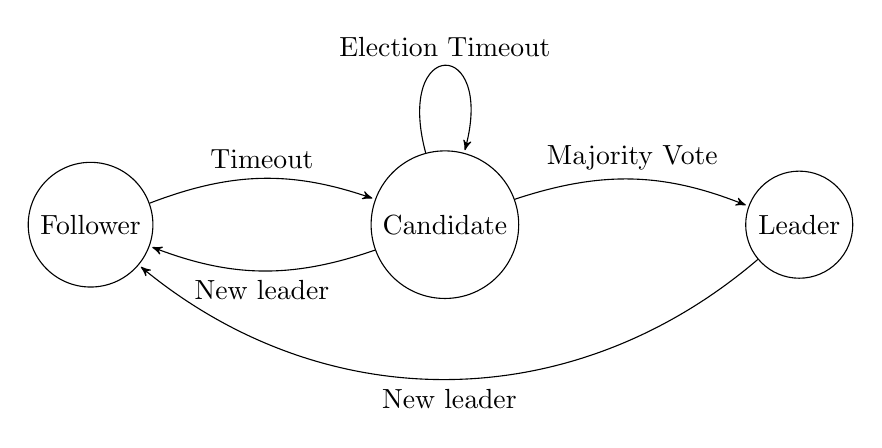
\begin{tikzpicture}[>=stealth',shorten >=1pt,auto,node distance=4.5cm]
  \node[state]  (f)                {Follower};
  \node[state]  (c) [right of=f]  {Candidate};
  \node[state]  (l) [right of=c]  {Leader};

  \path[->]          (f)  edge   [bend left=20]   node {Timeout} (c);
  \path[->]          (c)  edge   [bend left=20]   node {New leader} (f);

  \path[->]          (c)  edge   [bend left=20]   node {Majority Vote} (l);
  \path[->]          (l)  edge   [bend left=40]   node {New leader} (f);
  \path[->] (c) edge [loop above] node {Election Timeout} (c);

\end{tikzpicture}
\end{center}

\section{Spec}

The following implements the skeleton portion of the leader election
protocol:\newline

\begin{tla}
Init ==
    /\ state = [s \in Servers |-> "Follower"]
    /\ messages = {} 
    /\ voted_for = [s \in Servers |-> ""]
    /\ vote_granted = [s \in Servers |-> {}]
    /\ vote_requested = [s \in Servers |-> 0]
    /\ term = [s \in Servers |-> 0]

RequestVoteSet(i) == {
    [fSrc |-> i, fDst |-> s, fType |-> "RequestVoteReq", fTerm |-> term[i]] 
        : s \in Servers \ {i}
}

Campaign(i) == 
    /\ vote_requested[i] = 0
    /\ vote_requested' = [vote_requested EXCEPT ![i] = 1]
    /\ messages' = messages \cup RequestVoteSet(i) 
    /\ UNCHANGED <<state, term, vote_granted, voted_for>>

KeepAliveSet(i) == {
    [fSrc |-> i, fDst |-> s, fType |-> "AppendEntryReq", fTerm |-> term[i]] 
        : s \in Servers \ {i}
}

Leader(i) == 
    /\ state[i] = "Leader"
    /\ messages' = messages \cup KeepAliveSet(i) 
    /\ UNCHANGED <<state, voted_for, term, vote_granted, vote_requested>>

BecomeLeader(i) ==
    /\ Cardinality(vote_granted[i]) > Cardinality(Servers) \div 2
    /\ state' = [state EXCEPT ![i] = "Leader"]
    /\ UNCHANGED <<messages, voted_for, term, vote_granted, vote_requested>>

Candidate(i) == 
    /\ state[i] = "Candidate"
    /\ \/ Campaign(i)
       \/ BecomeLeader(i)
       \/ Timeout(i)

Follower(i) == 
    /\ state[i] = "Follower"
    /\ Timeout(i)

Receive(msg) == 
    \/ /\ msg.fType = "AppendEntryReq"
       /\ AppendEntryReq(msg) 
    \/ /\ msg.fType = "AppendEntryResp"
       /\ AppendEntryResp(msg) 
    \/ /\ msg.fType = "RequestVoteReq"
       /\ RequestVoteReq(msg) 
    \/ /\ msg.fType = "RequestVoteResp"
       /\ RequestVoteResp(msg) 

Next == 
    \/ \E i \in Servers : 
          \/ Leader(i) 
          \/ Candidate(i)
          \/ Follower(i)
    \/ \E msg \in messages : Receive(msg)
\end{tla}
\begin{tlatex}
\@x{ Init \.{\defeq}}%
 \@x{\@s{16.4} \.{\land} state \.{=} [ s \.{\in} Servers
 \.{\mapsto}\@w{Follower} ]}%
\@x{\@s{16.4} \.{\land} messages \.{=} \{ \}}%
 \@x{\@s{16.4} \.{\land} voted\_for \.{=} [ s \.{\in} Servers \.{\mapsto}\@w{}
 ]}%
 \@x{\@s{16.4} \.{\land} vote\_granted \.{=} [ s \.{\in} Servers \.{\mapsto}
 \{ \} ]}%
 \@x{\@s{16.4} \.{\land} vote\_requested \.{=} [ s \.{\in} Servers \.{\mapsto}
 0 ]}%
\@x{\@s{16.4} \.{\land} term \.{=} [ s \.{\in} Servers \.{\mapsto} 0 ]}%
\@pvspace{8.0pt}%
\@x{ RequestVoteSet ( i ) \.{\defeq} \{}%
 \@x{\@s{16.4} [ fSrc \.{\mapsto} i ,\, fDst \.{\mapsto} s ,\, fType
 \.{\mapsto}\@w{RequestVoteReq} ,\, fTerm \.{\mapsto} term [ i ] ]}%
\@x{\@s{31.47} \.{:} s \.{\in} Servers \.{\,\backslash\,} \{ i \}}%
\@x{ \}}%
\@pvspace{8.0pt}%
\@x{ Campaign ( i ) \.{\defeq}}%
\@x{\@s{16.4} \.{\land} vote\_requested [ i ] \.{=} 0}%
 \@x{\@s{16.4} \.{\land} vote\_requested \.{'} \.{=} [ vote\_requested
 {\EXCEPT} {\bang} [ i ] \.{=} 1 ]}%
 \@x{\@s{16.4} \.{\land} messages \.{'} \.{=} messages \.{\cup} RequestVoteSet
 ( i )}%
 \@x{\@s{16.4} \.{\land} {\UNCHANGED} {\langle} state ,\, term ,\,
 vote\_granted ,\, voted\_for {\rangle}}%
\@pvspace{8.0pt}%
\@x{ KeepAliveSet ( i ) \.{\defeq} \{}%
 \@x{\@s{16.4} [ fSrc \.{\mapsto} i ,\, fDst \.{\mapsto} s ,\, fType
 \.{\mapsto}\@w{AppendEntryReq} ,\, fTerm \.{\mapsto} term [ i ] ]}%
\@x{\@s{31.47} \.{:} s \.{\in} Servers \.{\,\backslash\,} \{ i \}}%
\@x{ \}}%
\@pvspace{8.0pt}%
\@x{ Leader ( i ) \.{\defeq}}%
\@x{\@s{16.4} \.{\land} state [ i ] \.{=}\@w{Leader}}%
 \@x{\@s{16.4} \.{\land} messages \.{'} \.{=} messages \.{\cup} KeepAliveSet (
 i )}%
 \@x{\@s{16.4} \.{\land} {\UNCHANGED} {\langle} state ,\, voted\_for ,\, term
 ,\, vote\_granted ,\, vote\_requested {\rangle}}%
\@pvspace{8.0pt}%
\@x{ BecomeLeader ( i ) \.{\defeq}}%
 \@x{\@s{16.4} \.{\land} Cardinality ( vote\_granted [ i ] ) \.{>} Cardinality
 ( Servers ) \.{\div} 2}%
 \@x{\@s{16.4} \.{\land} state \.{'} \.{=} [ state {\EXCEPT} {\bang} [ i ]
 \.{=}\@w{Leader} ]}%
 \@x{\@s{16.4} \.{\land} {\UNCHANGED} {\langle} messages ,\, voted\_for ,\,
 term ,\, vote\_granted ,\, vote\_requested {\rangle}}%
\@pvspace{8.0pt}%
\@x{ Candidate ( i ) \.{\defeq}}%
\@x{\@s{16.4} \.{\land} state [ i ] \.{=}\@w{Candidate}}%
\@x{\@s{16.4} \.{\land} \.{\lor} Campaign ( i )}%
\@x{\@s{27.51} \.{\lor} BecomeLeader ( i )}%
\@x{\@s{27.51} \.{\lor} Timeout ( i )}%
\@pvspace{8.0pt}%
\@x{ Follower ( i ) \.{\defeq}}%
\@x{\@s{16.4} \.{\land} state [ i ] \.{=}\@w{Follower}}%
\@x{\@s{16.4} \.{\land} Timeout ( i )}%
\@pvspace{8.0pt}%
\@x{ Receive ( msg ) \.{\defeq}}%
 \@x{\@s{16.4} \.{\lor}\@s{5.06} \.{\land} msg . fType
 \.{=}\@w{AppendEntryReq}}%
\@x{\@s{32.57} \.{\land} AppendEntryReq ( msg )}%
 \@x{\@s{16.4} \.{\lor}\@s{5.06} \.{\land} msg . fType
 \.{=}\@w{AppendEntryResp}}%
\@x{\@s{32.57} \.{\land} AppendEntryResp ( msg )}%
 \@x{\@s{16.4} \.{\lor}\@s{5.06} \.{\land} msg . fType
 \.{=}\@w{RequestVoteReq}}%
\@x{\@s{32.57} \.{\land} RequestVoteReq ( msg )}%
 \@x{\@s{16.4} \.{\lor}\@s{5.06} \.{\land} msg . fType
 \.{=}\@w{RequestVoteResp}}%
\@x{\@s{32.57} \.{\land} RequestVoteResp ( msg )}%
\@pvspace{8.0pt}%
\@x{ Next \.{\defeq}}%
\@x{\@s{16.4} \.{\lor} \E\, i \.{\in} Servers \.{:}}%
\@x{\@s{34.73} \.{\lor} Leader ( i )}%
\@x{\@s{34.73} \.{\lor} Candidate ( i )}%
\@x{\@s{34.73} \.{\lor} Follower ( i )}%
\@x{\@s{16.4} \.{\lor} \E\, msg \.{\in} messages \.{:} Receive ( msg )}%
\end{tlatex}

\begin{itemize}
    \item The Spec picks a server to make progress in \textit{Next}, including
    process messages with \textit{Receive}. \textit{Receive} handling is 
    state agnostic and implemented as such
    \item \textit{message} is defined to be a set to hold a collection of functions, where 
    each function is a message with source, destination, type, and more specified
    \item \textit{voted\_for} represents who a node has previously voted for. This is to 
    prevent a node from voting more than once
    \item \textit{vote\_granted} tracks how many peers have voted for a node
    \item \textit{vote\_requested} tracks if a node has already issued request vote
    \item The actions defined for every state reflect description earlier 
    \item \textit{Follower} either Receive or Timeout and campaign to be a leader
    \item \textit{Candidate} campaigns to be a leader, and becomes one if it has
    enough vote. Failing to collect enough votes, \textit{Candidate} start a new
    term of election. It can also receive a request with a higher term and
    transition to be a \textit{Follower}.
\end{itemize}


The message processing functions are fairly similar in structure, here we will
take a look at \textit{RequestVoteReq}:\newline

\begin{tla}
RequestVoteReq(msg) == 
    LET 
        i == msg.fDst
        j == msg.fSrc
        type == msg.fType
        t == msg.fTerm
    IN 
        \* haven't voted, or whom we voted re-requested
        \/ /\ t = term[i]
           /\ \/ voted_for[i] = j 
              \/ voted_for[i] = ""
           /\ voted_for' = [voted_for EXCEPT ![i] = j]
           /\ messages' = AddMessage([fSrc |-> i, 
                                        fDst |-> j, 
                                        fType |-> "RequestVoteResp",
                                        fTerm |-> t, 
                                        fSuccess |-> 1],
                                        RemoveMessage(msg, messages))
           /\ UNCHANGED <<state, term, vote_granted, vote_requested, establish_leadership >>
        \* already voted someone else
        \/ /\ t = term[i]
           /\ voted_for[i] # j 
           /\ voted_for[i] # ""
           /\ messages' = AddMessage([fSrc |-> i, 
                                        fDst |-> j, 
                                        fType |-> "RequestVoteResp",
                                        fTerm |-> t, 
                                        fSuccess |-> 0],
                                        RemoveMessage(msg, messages))
            /\ UNCHANGED <<state, voted_for, term, vote_granted, vote_requested, establish_leadership>>
        \/  /\ t < term[i]
            /\ messages' = AddMessage([fSrc |-> i, 
                                        fDst |-> j, 
                                        fType |-> "RequestVoteResp",
                                        fTerm |-> term[i], 
                                        fSuccess |-> 0],
                                        RemoveMessage(msg, messages))
            /\ UNCHANGED <<state, voted_for, term, vote_granted, vote_requested, establish_leadership>>
        \* revert back to follower
        \/  /\ t > term[i]
            /\ state' = [state EXCEPT ![i] = "Follower"]
            /\ term' = [term EXCEPT ![i] = t]
            /\ voted_for' = [voted_for EXCEPT ![i] = j]
            /\ vote_granted' = [vote_granted EXCEPT ![i] = {}]
            /\ vote_requested' = [vote_requested EXCEPT ![i] = 0]
            /\ establish_leadership' = [establish_leadership EXCEPT ![i] = 0]
            /\ messages' = AddMessage([fSrc |-> i, 
                                        fDst |-> j, 
                                        fType |-> "RequestVoteResp",
                                        fTerm |-> t, 
                                        fSuccess |-> 1],
                                        RemoveMessage(msg, messages))
\end{tla}
\begin{tlatex}
\@x{ RequestVoteReq ( msg ) \.{\defeq}}%
\@x{\@s{16.4} \.{\LET}}%
\@x{\@s{32.8} i\@s{0.42} \.{\defeq} msg . fDst}%
\@x{\@s{32.8} j \.{\defeq} msg . fSrc}%
\@x{\@s{32.8} type \.{\defeq} msg . fType}%
\@x{\@s{32.8} t \.{\defeq} msg . fTerm}%
\@x{\@s{16.4} \.{\IN}}%
\@x{\@s{32.8}}%
\@y{%
  haven't voted, or whom we voted re-requested
}%
\@xx{}%
\@x{\@s{32.8} \.{\lor} \.{\land} t \.{=} term [ i ]}%
\@x{\@s{43.91} \.{\land} \.{\lor} voted\_for [ i ] \.{=} j}%
\@x{\@s{55.02} \.{\lor} voted\_for [ i ] \.{=}\@w{}}%
 \@x{\@s{43.91} \.{\land} voted\_for \.{'} \.{=} [ voted\_for {\EXCEPT}
 {\bang} [ i ] \.{=} j ]}%
 \@x{\@s{43.91} \.{\land} messages \.{'} \.{=} AddMessage ( [ fSrc \.{\mapsto}
 i ,\,}%
\@x{\@s{180.15} fDst \.{\mapsto} j ,\,}%
\@x{\@s{180.15} fType\@s{2.95} \.{\mapsto}\@w{RequestVoteResp} ,\,}%
\@x{\@s{180.15} fTerm \.{\mapsto} t ,\,}%
\@x{\@s{180.15} fSuccess \.{\mapsto} 1 ] ,\,}%
\@x{\@s{180.15} RemoveMessage ( msg ,\, messages ) )}%
 \@x{\@s{43.91} \.{\land} {\UNCHANGED} {\langle} state ,\, term ,\,
 vote\_granted ,\, vote\_requested ,\, establish\_leadership {\rangle}}%
\@x{\@s{32.8}}%
\@y{%
  already voted someone else
}%
\@xx{}%
\@x{\@s{32.8} \.{\lor} \.{\land} t \.{=} term [ i ]}%
\@x{\@s{43.91} \.{\land} voted\_for [ i ] \.{\neq} j}%
\@x{\@s{43.91} \.{\land} voted\_for [ i ] \.{\neq}\@w{}}%
 \@x{\@s{43.91} \.{\land} messages \.{'} \.{=} AddMessage ( [ fSrc \.{\mapsto}
 i ,\,}%
\@x{\@s{180.15} fDst \.{\mapsto} j ,\,}%
\@x{\@s{180.15} fType\@s{2.95} \.{\mapsto}\@w{RequestVoteResp} ,\,}%
\@x{\@s{180.15} fTerm \.{\mapsto} t ,\,}%
\@x{\@s{180.15} fSuccess \.{\mapsto} 0 ] ,\,}%
\@x{\@s{180.15} RemoveMessage ( msg ,\, messages ) )}%
 \@x{\@s{48.01} \.{\land} {\UNCHANGED} {\langle} state ,\, voted\_for ,\, term
 ,\, vote\_granted ,\, vote\_requested ,\, establish\_leadership {\rangle}}%
\@x{\@s{32.8} \.{\lor}\@s{4.1} \.{\land} t \.{<} term [ i ]}%
 \@x{\@s{48.01} \.{\land} messages \.{'} \.{=} AddMessage ( [ fSrc \.{\mapsto}
 i ,\,}%
\@x{\@s{180.15} fDst \.{\mapsto} j ,\,}%
\@x{\@s{180.15} fType\@s{2.95} \.{\mapsto}\@w{RequestVoteResp} ,\,}%
\@x{\@s{180.15} fTerm \.{\mapsto} term [ i ] ,\,}%
\@x{\@s{180.15} fSuccess \.{\mapsto} 0 ] ,\,}%
\@x{\@s{180.15} RemoveMessage ( msg ,\, messages ) )}%
 \@x{\@s{48.01} \.{\land} {\UNCHANGED} {\langle} state ,\, voted\_for ,\, term
 ,\, vote\_granted ,\, vote\_requested ,\, establish\_leadership {\rangle}}%
\@x{\@s{32.8}}%
\@y{%
  revert back to follower
}%
\@xx{}%
\@x{\@s{32.8} \.{\lor}\@s{4.1} \.{\land} t \.{>} term [ i ]}%
 \@x{\@s{48.01} \.{\land} state \.{'} \.{=} [ state {\EXCEPT} {\bang} [ i ]
 \.{=}\@w{Follower} ]}%
 \@x{\@s{48.01} \.{\land} term \.{'} \.{=} [ term {\EXCEPT} {\bang} [ i ]
 \.{=} t ]}%
 \@x{\@s{48.01} \.{\land} voted\_for \.{'} \.{=} [ voted\_for {\EXCEPT}
 {\bang} [ i ] \.{=} j ]}%
 \@x{\@s{48.01} \.{\land} vote\_granted \.{'} \.{=} [ vote\_granted {\EXCEPT}
 {\bang} [ i ] \.{=} \{ \} ]}%
 \@x{\@s{48.01} \.{\land} vote\_requested \.{'} \.{=} [ vote\_requested
 {\EXCEPT} {\bang} [ i ] \.{=} 0 ]}%
 \@x{\@s{48.01} \.{\land} establish\_leadership \.{'} \.{=} [
 establish\_leadership {\EXCEPT} {\bang} [ i ] \.{=} 0 ]}%
 \@x{\@s{48.01} \.{\land} messages \.{'} \.{=} AddMessage ( [ fSrc \.{\mapsto}
 i ,\,}%
\@x{\@s{180.15} fDst \.{\mapsto} j ,\,}%
\@x{\@s{180.15} fType\@s{2.95} \.{\mapsto}\@w{RequestVoteResp} ,\,}%
\@x{\@s{180.15} fTerm \.{\mapsto} t ,\,}%
\@x{\@s{180.15} fSuccess \.{\mapsto} 1 ] ,\,}%
\@x{\@s{180.15} RemoveMessage ( msg ,\, messages ) )}%
\end{tlatex}
\newline

The handling is basically split into three cases. If received request is on a
higher term, processing node grants vote and becomes a Follower. If received
request is on a lower term, processing node ignores request. If received request
is on the same term, then processing node grants vote if it hasn't voted, or had
voted for the requester prior.

\section{Simplify Model}

TLC will run the Spec as defined, but due to the expoential growth of states it
is unlikely to complete in a practical amount of time. We need to simplify the
model to allow the model checker completes in a reasonable time, but possibly
trades off some correctness. Careful consideration must go into finding the
right balance between maximizing model correctness and minimizing model checker
runtime.\newline

The main strategy is to \textit{bound} the state graph. The following describe a
set of optimization applied for this example.

\subsection{Modeling Messages as a Set}

In the original Raft TLA+ Spec \cite{raft_tla}, messages are modelled as an
\textit{unordered map} to track the count of each message. It is possible for a
sender to repeatedly send the same message (eg. keepalive), and grows the 
message count in an unbounded fashion.\newline

\textit{messages} in this example has been implemented as a set so the model 
checker doesn't go into the weeds as the count of a message grows. It is still 
possible for messages to grow unboundedly because the message carries a term
value. Further changes are described below.

\subsection{Limit Term Divergence} 

It is possible for the a node to \textit{never} make progress (eg. one node is
somehow partitioned off and the rest of the cluster keeps moving onto newer
terms). While we do want to exercise handling of diverging terms in a cluster,
limiting the range of terms in the cluster likely doesn't reduce the coverage by
much.  We can limit divergence by preventing a node with a high term value to go
into election. This allows the nodes with low term value to catchup. and thus
reduce the number of states in the graph.\newline

We can include \textit{LimitDivergence} as a conjunction in
\textit{Timeout}:\newline
\begin{tla}
LimitDivergence(i) == 
    LET 
        values == {term[s] : s \in Servers}
        max_v == CHOOSE x \in values : \A y \in values : x >= y
        min_v == CHOOSE x \in values : \A y \in values : x <= y
    IN 
        \/ /\ term[i] # max_v
        \/ /\ term[i] = max_v 
           /\ term[i] - min_v < MaxDiff

Timeout(i) == 
    /\ LimitDivergence(i)
    /\ state' = [state EXCEPT ![i] = "Candidate"]
    /\ voted_for' = [voted_for EXCEPT ![i] = i]             \* voted for myself
    /\ vote_granted' = [vote_granted EXCEPT ![i] = {i}]
    /\ vote_requested' = [vote_requested EXCEPT ![i] = 0]
    /\ term' = [term EXCEPT ![i] = @ + 1]                   \* bump term
    /\ establish_leadership' = [establish_leadership EXCEPT ![i] = 0]
    /\ UNCHANGED <<messages>>
    \* /\ PrintT(state')
\end{tla}
\begin{tlatex}
\@x{ LimitDivergence ( i ) \.{\defeq}}%
\@x{\@s{16.4} \.{\LET}}%
\@x{\@s{32.8} values \.{\defeq} \{ term [ s ] \.{:} s \.{\in} Servers \}}%
 \@x{\@s{32.8} max\_v \.{\defeq} {\CHOOSE} x \.{\in} values \.{:} \A\, y
 \.{\in} values \.{:} x \.{\geq} y}%
 \@x{\@s{32.8} min\_v\@s{1.49} \.{\defeq} {\CHOOSE} x \.{\in} values \.{:}
 \A\, y \.{\in} values \.{:} x \.{\leq} y}%
\@x{\@s{16.4} \.{\IN}}%
\@x{\@s{32.8} \.{\lor} \.{\land} term [ i ] \.{\neq} max\_v}%
\@x{\@s{32.8} \.{\lor} \.{\land} term [ i ] \.{=} max\_v}%
\@x{\@s{43.91} \.{\land} term [ i ] \.{-} min\_v \.{<} MaxDiff}%
\@pvspace{8.0pt}%
\@x{ Timeout ( i ) \.{\defeq}}%
\@x{\@s{16.4} \.{\land}\@s{9.72} LimitDivergence ( i )}%
 \@x{\@s{16.4} \.{\land}\@s{9.72} state \.{'} \.{=} [ state {\EXCEPT} {\bang}
 [ i ] \.{=}\@w{Candidate} ]}%
 \@x{\@s{16.4} \.{\land}\@s{9.72} voted\_for \.{'} \.{=} [ voted\_for
 {\EXCEPT} {\bang} [ i ] \.{=} i ]\@s{49.19}}%
\@y{%
  voted for myself
}%
\@xx{}%
 \@x{\@s{16.4} \.{\land}\@s{9.72} vote\_granted \.{'} \.{=} [ vote\_granted
 {\EXCEPT} {\bang} [ i ] \.{=} \{ i \} ]}%
 \@x{\@s{16.4} \.{\land}\@s{9.72} vote\_requested \.{'} \.{=} [
 vote\_requested {\EXCEPT} {\bang} [ i ] \.{=} 0 ]}%
 \@x{\@s{16.4} \.{\land}\@s{9.72} term \.{'} \.{=} [ term {\EXCEPT} {\bang} [
 i ] \.{=} @ \.{+} 1 ]\@s{68.59}}%
\@y{%
  bump term
}%
\@xx{}%
 \@x{\@s{16.4} \.{\land}\@s{9.72} establish\_leadership \.{'} \.{=} [
 establish\_leadership {\EXCEPT} {\bang} [ i ] \.{=} 0 ]}%
\@x{\@s{16.4} \.{\land}\@s{9.72} {\UNCHANGED} {\langle} messages {\rangle}}%
\@x{\@s{16.4}}%
\@y{%
  /\ PrintT(state')
}%
\@xx{}%
\end{tlatex}

\subsection{Normalize Cluster Term}

However, term \textit{itself} can grow unbounded. This is a key tenent 
converging protocols rely on, an monotonically increasing counter. We want to 
\textit{normalize} the range of terms in the cluster so the minimum value is
reset back to 0. This provides an upper bound to the state graph.\newline

\begin{tla}
Normalize == 
    LET 
        values == {term[s] : s \in Servers}
        max_v == CHOOSE x \in values : \A y \in values : x >= y
        min_v == CHOOSE x \in values : \A y \in values : x <= y
    IN 
        /\ max_v = MaxTerm
        /\ term' = [s \in Servers |-> term[s] - min_v]
        /\ messages' = {}
        /\ UNCHANGED <<state, voted_for, vote_granted, vote_requested, establish_leadership>>

Next == 
    \/ /\ \A i \in Servers : term[i] # MaxTerm 
       /\ \/ \E i \in Servers : 
                \/ Leader(i) 
                \/ Candidate(i)
                \/ Follower(i)
          \/ \E msg \in messages : Receive(msg)
    \/ /\ \E i \in Servers: term[i] = MaxTerm 
       /\ Normalize
\end{tla}
\begin{tlatex}
\@x{ Normalize \.{\defeq}}%
\@x{\@s{16.4} \.{\LET}}%
\@x{\@s{32.8} values \.{\defeq} \{ term [ s ] \.{:} s \.{\in} Servers \}}%
 \@x{\@s{32.8} max\_v \.{\defeq} {\CHOOSE} x \.{\in} values \.{:} \A\, y
 \.{\in} values \.{:} x \.{\geq} y}%
 \@x{\@s{32.8} min\_v\@s{1.49} \.{\defeq} {\CHOOSE} x \.{\in} values \.{:}
 \A\, y \.{\in} values \.{:} x \.{\leq} y}%
\@x{\@s{16.4} \.{\IN}}%
\@x{\@s{32.8} \.{\land} max\_v \.{=} MaxTerm}%
 \@x{\@s{32.8} \.{\land} term \.{'}\@s{5.41} \.{=} [ s \.{\in} Servers
 \.{\mapsto} term [ s ] \.{-} min\_v ]}%
\@x{\@s{32.8} \.{\land} messages \.{'} \.{=} \{ \}}%
 \@x{\@s{32.8} \.{\land} {\UNCHANGED} {\langle} state ,\, voted\_for ,\,
 vote\_granted ,\, vote\_requested ,\, establish\_leadership {\rangle}}%
\@pvspace{8.0pt}%
\@x{ Next \.{\defeq}}%
 \@x{\@s{16.4} \.{\lor} \.{\land} \A\, i \.{\in} Servers \.{:} term [ i ]
 \.{\neq} MaxTerm}%
\@x{\@s{27.51} \.{\land} \.{\lor} \E\, i \.{\in} Servers \.{:}}%
\@x{\@s{56.95} \.{\lor} Leader ( i )}%
\@x{\@s{56.95} \.{\lor} Candidate ( i )}%
\@x{\@s{56.95} \.{\lor} Follower ( i )}%
\@x{\@s{38.62} \.{\lor} \E\, msg \.{\in} messages \.{:} Receive ( msg )}%
 \@x{\@s{16.4} \.{\lor} \.{\land} \E\, i \.{\in} Servers \.{:} term [ i ]
 \.{=} MaxTerm}%
\@x{\@s{27.51} \.{\land} Normalize}%
\end{tlatex}
\newline

The implementation ensures only the state machine only moves forward when none
of the nodes is on MaxTerm. If any of the node is on MaxTerm, the cluster terms
are normalized.\newline

Another caveat here is in the initial implementation I didn't update messsages.
This led to liveness property violation as the messages had terms disagreeing
with the system state. To simplify the Spec I simply cleared all messages. This 
indirectly verifies a portion of the packet loss handling in the Spec.

\subsection{Send Requests to Cluster as a Set}

Initially the send requests are implemented using the existential quantifier. 
This introduces many interleaving states. This was latter replaced with a
universal quantifier so the set of messages are only sent once. The
implementation no longer tracks if the responses were received, since the 
Spec should handle packet loss scenarios as well.\newline

\begin{tla}
RequestVoteSet(i) == {
    [fSrc |-> i, fDst |-> s, fType |-> "RequestVoteReq", fTerm |-> term[i]] 
        : s \in Servers \ {i}
}

Campaign(i) == 
    /\ vote_requested[i] = 0
    /\ vote_requested' = [vote_requested EXCEPT ![i] = 1]
    /\ messages' = messages \cup RequestVoteSet(i) 
    /\ UNCHANGED <<state, term, vote_granted, voted_for, establish_leadership>>

KeepAliveSet(i) == {
    [fSrc |-> i, fDst |-> s, fType |-> "AppendEntryReq", fTerm |-> term[i]] 
        : s \in Servers \ {i}
}

Leader(i) == 
    /\ state[i] = "Leader"
    /\ establish_leadership[i] = 0
    /\ establish_leadership' = [establish_leadership EXCEPT ![i] = 1]
    /\ messages' = messages \cup KeepAliveSet(i) 
    /\ UNCHANGED <<state, voted_for, term, vote_granted, vote_requested>>
\end{tla}
\begin{tlatex}
\@x{ RequestVoteSet ( i ) \.{\defeq} \{}%
 \@x{\@s{16.4} [ fSrc \.{\mapsto} i ,\, fDst \.{\mapsto} s ,\, fType
 \.{\mapsto}\@w{RequestVoteReq} ,\, fTerm \.{\mapsto} term [ i ] ]}%
\@x{\@s{31.47} \.{:} s \.{\in} Servers \.{\,\backslash\,} \{ i \}}%
\@x{ \}}%
\@pvspace{8.0pt}%
\@x{ Campaign ( i ) \.{\defeq}}%
\@x{\@s{16.4} \.{\land} vote\_requested [ i ] \.{=} 0}%
 \@x{\@s{16.4} \.{\land} vote\_requested \.{'} \.{=} [ vote\_requested
 {\EXCEPT} {\bang} [ i ] \.{=} 1 ]}%
 \@x{\@s{16.4} \.{\land} messages \.{'} \.{=} messages \.{\cup} RequestVoteSet
 ( i )}%
 \@x{\@s{16.4} \.{\land} {\UNCHANGED} {\langle} state ,\, term ,\,
 vote\_granted ,\, voted\_for ,\, establish\_leadership {\rangle}}%
\@pvspace{8.0pt}%
\@x{ KeepAliveSet ( i ) \.{\defeq} \{}%
 \@x{\@s{16.4} [ fSrc \.{\mapsto} i ,\, fDst \.{\mapsto} s ,\, fType
 \.{\mapsto}\@w{AppendEntryReq} ,\, fTerm \.{\mapsto} term [ i ] ]}%
\@x{\@s{31.47} \.{:} s \.{\in} Servers \.{\,\backslash\,} \{ i \}}%
\@x{ \}}%
\@pvspace{8.0pt}%
\@x{ Leader ( i ) \.{\defeq}}%
\@x{\@s{16.4} \.{\land} state [ i ] \.{=}\@w{Leader}}%
\@x{\@s{16.4} \.{\land} establish\_leadership [ i ] \.{=} 0}%
 \@x{\@s{16.4} \.{\land} establish\_leadership \.{'} \.{=} [
 establish\_leadership {\EXCEPT} {\bang} [ i ] \.{=} 1 ]}%
 \@x{\@s{16.4} \.{\land} messages \.{'} \.{=} messages \.{\cup} KeepAliveSet (
 i )}%
 \@x{\@s{16.4} \.{\land} {\UNCHANGED} {\langle} state ,\, voted\_for ,\, term
 ,\, vote\_granted ,\, vote\_requested {\rangle}}%
\end{tlatex}

\subsection{Prune Messages with Stale Terms}

When a node's term advances, it'll discard all messages targeted to it with
older terms. Keeping messages with stale terms allows the model checker to 
verify the node correctly discards them, but can exponentially grow the state
machine. To simplify the model, we can prune stale messages as we add a new 
message: \newline

\begin{tla}
AddMessage(to_add, msgs) == 
    LET 
        pruned == {msg \in msgs : 
                    ~(msg.fDst = to_add.fDst /\ msg.fTerm < to_add.fTerm)}
    IN
        pruned \cup {to_add}

RemoveMessage(to_remove, msgs) ==
\end{tla}
\begin{tlatex}
\@x{ AddMessage ( to\_add ,\, msgs ) \.{\defeq}}%
\@x{\@s{16.4} \.{\LET}}%
\@x{\@s{32.8} pruned \.{\defeq} \{ msg \.{\in} msgs \.{:}}%
 \@x{\@s{91.33} {\lnot} ( msg . fDst \.{=} to\_add . fDst \.{\land} msg .
 fTerm \.{<} to\_add . fTerm ) \}}%
\@x{\@s{16.4} \.{\IN}}%
\@x{\@s{32.8} pruned \.{\cup} \{ to\_add \}}%
\@pvspace{8.0pt}%
\@x{ RemoveMessage ( to\_remove ,\, msgs ) \.{\defeq}}%
\end{tlatex}

\section{Safety}

One of the goals for the protocol is to ensure the cluster only have one leader.
It is possible for the clusters to have mulitple leaders due to unfavourable
network connections. For example, a leader node is partitioned off and a new
leader is elected. However, even when the cluster have mutliple leaders, they
must be on different terms. The leader with the highest term is effectively the
\textit{true leader}. This invariant can be implemented like so:\newline

\begin{tla}
LeaderUniqueTerm ==
    \A s1, s2 \in Servers :
        (state[s1] = "Leader" /\ state[s2] = "Leader" /\ s1 /= s2) => (term[s1] # term[s2])
\end{tla}
\begin{tlatex}
\@x{ LeaderUniqueTerm \.{\defeq}}%
\@x{\@s{16.4} \A\, s1 ,\, s2 \.{\in} Servers \.{:}}%
 \@x{\@s{27.72} ( state [ s1 ] \.{=}\@w{Leader} \.{\land} state [ s2 ]
 \.{=}\@w{Leader} \.{\land} s1 \.{\neq} s2 ) \.{\implies} ( term [ s1 ]
 \.{\neq} term [ s2 ] )}%
\end{tlatex}
\newline

For every pair of nodes, they cannot both be Leaders and have the same
term.

\section{Liveness}

In any failure recovery scenario, the nodes in the cluster converges to a higher
term value either voluntary or involuntarily. The following is a few ways:
\begin{itemize}
    \item A node timed out and starts a new election on a new term 
    \item A partitioned follower receives heartbeat from a new leader on a new term
    \item A candidate receiving a request vote from another candidate on a higher term
\end{itemize}

In any case, a node's term number always increase. This can be described as below:\newline
\begin{tla}
Converge ==
    \A s \in Servers:
        term[s] = 0 ~> term[s] = MaxTerm - MaxDiff
\end{tla}
\begin{tlatex}
\@x{ Converge \.{\defeq}}%
\@x{\@s{16.4} \A\, s \.{\in} Servers \.{:}}%
 \@x{\@s{27.72} term [ s ] \.{=} 0 \.{\leadsto} term [ s ] \.{=} MaxTerm \.{-}
 MaxDiff}%
\end{tlatex}
\newline

Instead of MaxTerm, we use MaxTerm-MaxDiff to account to ensure the liveness
property is always upheld even after Normalization. However, running the Spec
against TLC now will encounter a set of stuttering issues. We also need to
update the fairness description to the Spec to ensure all possible actions are
called when the enabling conditions are \textit{eventually always} true:\newline

\begin{tla}
Liveness == 
    /\ \A i \in Servers : 
        /\ WF_vars(Leader(i))
        /\ WF_vars(Candidate(i))
        /\ WF_vars(Follower(i))
    /\ WF_vars(\E msg \in messages : Receive(msg))
\end{tla}
\begin{tlatex}
\@x{ Liveness \.{\defeq}}%
\@x{\@s{16.4} \.{\land} \A\, i \.{\in} Servers \.{:}}%
\@x{\@s{31.61} \.{\land} {\WF}_{ vars} ( Leader ( i ) )}%
\@x{\@s{31.61} \.{\land} {\WF}_{ vars} ( Candidate ( i ) )}%
\@x{\@s{31.61} \.{\land} {\WF}_{ vars} ( Follower ( i ) )}%
 \@x{\@s{16.4} \.{\land} {\WF}_{ vars} ( \E\, msg \.{\in} messages \.{:}
 Receive ( msg ) )}%
\end{tlatex}

SPECIFICATION Spec

INVARIANTS 
    \* TypeOK
PROPERTIES 
    \* Liveness


\section{Requirement}

\section{Spec}

\begin{tla}
Init ==
    /\ lastHash = NoHash
    /\ distributedLedger = [n \in Node |-> [h \in Hash |-> NoBlock]]
    /\ received = [n \in Node |-> {}]
\end{tla}
\begin{tlatex}
\@x{ Init \.{\defeq}}%
\@x{\@s{16.4} \.{\land} lastHash \.{=} NoHash}%
 \@x{\@s{16.4} \.{\land} distributedLedger \.{=} [ n \.{\in} Node \.{\mapsto}
 [ h \.{\in} Hash \.{\mapsto} NoBlock ] ]}%
\@x{\@s{16.4} \.{\land} received \.{=} [ n \.{\in} Node \.{\mapsto} \{ \} ]}%
\end{tlatex}
\newline

\begin{itemize}
    \item Every node is a ledger in this system, initialized to NoBlock
    \item Every node's received set is initialized to nothing
\end{itemize}

\part{Examples with PlusCal}

\chapter{SPSC Lockfree Queue}

Single producer single consumer (SPSC) \textit{Lockfree} queue is a standard
data exchange queue between a producer and a consumer. The SPSC lockfree queue
promises data can exchange between producer and consumer in a \textit{lockfree}
fashion, suggesting all condition both producer and consumer can make
progress.\newline

Contrast to standard shared queues, a SPSC waitfree queue doesn't require the
use of a \textit{lock} (eg. mutex). The queue can be logically represented
fairly simply as:

\begin{lstlisting}
    template <typename T, ssize_t N>
    class cQueue<T> { 
        ssize_t rptr = 0; 
        ssize_t wptr = 0; 
        std::array<T, N> buffer;
        /* TODO: API definition below... */
    };
\end{lstlisting}

A real implementation need to account for memory ordering effects specific to
the architecture. For example, ARM has weak memory ordering model where
read/write may appear out of order between CPUs. In this chapter we will only
assume \textit{logical} execution where each command is issued sequentially
(even perceived across CPUs) to focus the discussion on TLA+.
\section{Requirement}

As mentioned in earlier section, a SPSC queue is represented by an array, a pair
of read write pointer. The implementation is (hopefully) descriptively trivial:

\begin{itemize}
    \item Two executing context, reader and writer
    \item Writer advances wtpr after writes
    \item Reader advances rtpr after reads
    \item If rtpr equals wptr, queue is empty
    \item If (wtpr + 1) \% N equals rptr, queue is full
\end{itemize}
% \newline

A possible implementation may look like below (not accounting for memory
ordering effects):
\begin{lstlisting}
    template <typename T, ssize_t N>
    class cQueue { 
        ssize_t rptr = 0;
        ssize_t wptr = 0; 
        std::array<T, N> buffer;

    public:
        bool read(T &v) { 
            /* queue empty check */
            if (rptr == wptr) { 
                return false;
            }
            /* data get */
            v = buffer[rptr]; 
            /* rtpr update */
            rptr = (rptr + 1) % N;
            return true;
        }

        bool write(const T &v) { 
            /* queue full check */
            if ((wptr + 1) % N == rptr) { 
                return false;
            }
            /* data write */
            buffer[wptr] = v;
            /* wptr update */
            wptr = (wptr + 1) % N;
            return true;
        }
    };
\end{lstlisting}

Since reader and writer execute in different context, the instructions in read
and write can interleave in \textit{any} way imaginable:
\begin{itemize}
    \item queue empty check can happen before or after queue full check
    \item data write happens immediately before data read
    \item ... so on and so forth
\end{itemize}

The key observations is that buffer[wtpr] is reserved by the producer.
buffer[wtpr] is either unused or being written to. In either case the reader is
not allowed to access it. Symmetric reasoning applies to rptr. This provides
the \textit{safety} to the design - but how do we verify this?\newline

This is where TLA+ can help us formally verify the design.

\section{Spec}

TLA+ specification can be writen using its native formal specification
language, or a C-like syntax called PlusCal (which transpiles down to itse
native form). In this example, I chose to implement the specification using
PlusCal, since the content to be verified is psuedo implementation. While it is
possible specify SPSC in native TLA+, it is the author's opinion that it is
more error prone in this case, each line is effective an individual state needs
to be modeled.\newline

The following is a snippet of the specification written in PlusCal, hopefully
intuitive to read:
\begin{ppcal}
procedure reader(i) 
variable 
begin
r_chk_empty:        if rptr = wptr then 
r_early_ret:            return;
                    end if;
r_read_buf:         assert buffer[rptr] # 0;
r_cs:               buffer[rptr] := 0;
r_upd_rtpr:         rptr := (rptr + 1) % N;
                    return;
end procedure; 

procedure writer(i) begin
w_chk_full:         if (wptr + 1) % N = rptr then 
w_early_ret:            return; 
                    end if;
w_write_buf:        assert buffer[wptr] = 0;
w_cs:               buffer[wptr] := wptr + 1000;
w_upd_wptr:         wptr := (wptr + 1) % N;
                    return;
end procedure; 
\end{ppcal}\newline
\begin{tlatex}
\@x{ {\p@procedure} reader ( i )}%
\@x{ {\p@variable}}%
\@x{ {\p@begin}}%
 \@x{ r\_chk\_empty\@s{.5}\textrm{:}\@s{3}\@s{28.7} {\p@if} rptr \.{=} wptr
 {\p@then}}%
 \@x{ r\_early\_ret\@s{.5}\textrm{:}\@s{3}\@s{51.39} {\p@return}
 {\p@semicolon}}%
\@x{\@s{91.60} {\p@end} {\p@if} {\p@semicolon}}%
 \@x{ r\_read\_buf\@s{.5}\textrm{:}\@s{3}\@s{36.83} {\p@assert} buffer [ rptr
 ] \.{\neq} 0 {\p@semicolon}}%
 \@x{ r\_cs\@s{.5}\textrm{:}\@s{3}\@s{66.02} buffer [ rptr ] \.{:=} 0
 {\p@semicolon}}%
 \@x{ r\_upd\_rtpr\@s{.5}\textrm{:}\@s{3}\@s{36.98} rptr \.{:=} ( rptr \.{+} 1
 ) \.{\%} N {\p@semicolon}}%
\@x{\@s{91.60} {\p@return} {\p@semicolon}}%
\@x{ {\p@end} {\p@procedure} {\p@semicolon}}%
\@pvspace{8.0pt}%
\@x{ {\p@procedure} writer ( i ) {\p@begin}}%
 \@x{ w\_chk\_full\@s{.5}\textrm{:}\@s{3}\@s{35.97} {\p@if} ( wptr \.{+} 1 )
 \.{\%} N \.{=} rptr {\p@then}}%
 \@x{ w\_early\_ret\@s{.5}\textrm{:}\@s{3}\@s{45.1} {\p@return}
 {\p@semicolon}}%
\@x{\@s{89.45} {\p@end} {\p@if} {\p@semicolon}}%
 \@x{ w\_write\_buf\@s{.5}\textrm{:}\@s{3}\@s{28.7} {\p@assert} buffer [ wptr
 ] \.{=} 0 {\p@semicolon}}%
 \@x{ w\_cs\@s{.5}\textrm{:}\@s{3}\@s{64.27} buffer [ wptr ] \.{:=} wptr \.{+}
 1000 {\p@semicolon}}%
 \@x{ w\_upd\_wptr\@s{.5}\textrm{:}\@s{3}\@s{32.8} wptr \.{:=} ( wptr \.{+} 1
 ) \.{\%} N {\p@semicolon}}%
\@x{\@s{92.28} {\p@return} {\p@semicolon}}%
\@x{ {\p@end} {\p@procedure} {\p@semicolon}}%
\end{tlatex}

Note each command starts with a \textit{label}, such as r\_chk\_empty. All the
actions associated with the label is assumed executed atomically. This is
reflected in the generated TLA+ code:
\begin{tla}
    r_chk_empty(self) == /\ pc[self] = "r_chk_empty"
                     /\ IF rptr = wptr
                           THEN /\ pc' = [pc EXCEPT ![self] = "r_early_ret"]
                           ELSE /\ pc' = [pc EXCEPT ![self] = "r_read_buf"]
                     /\ UNCHANGED << rptr, wptr, buffer, stack, i_, i >>
\end{tla}
\begin{tlatex}
 \@x{\@s{16.4} r\_chk\_empty ( self ) \.{\defeq} \.{\land} pc [ self ]
 \.{=}\@w{r\_chk\_empty}}%
\@x{\@s{97.45} \.{\land} {\IF} rptr \.{=} wptr}%
 \@x{\@s{120.71} \.{\THEN} \.{\land} pc \.{'} \.{=} [ pc {\EXCEPT} {\bang} [
 self ] \.{=}\@w{r\_early\_ret} ]}%
 \@x{\@s{120.71} \.{\ELSE} \.{\land} pc \.{'} \.{=} [ pc {\EXCEPT} {\bang} [
 self ] \.{=}\@w{r\_read\_buf} ]}%
 \@x{\@s{97.45} \.{\land} {\UNCHANGED} {\langle} rptr ,\, wptr ,\, buffer ,\,
 stack ,\, i\_ ,\, i {\rangle}}%
\end{tlatex}

\section{Safety}

As mentioned before, safety properties need to hold true in every single state.
Some safety requirement we can enforce, for example:\newline

Reader and writer cannot access the same index at the same time:
\begin{equation}
    \sim ((pc[100] = "w\_cs") \land (pc[101] = "r\_cs") \land rptr = wptr)
\end{equation}

All unused index should be set to 0:
\begin{equation}
    \A kk \in unused : buffer[kk] = 0
\end{equation}

At any given moment, buffer[wtpr] may be unused or written. buffer[rptr] may be
unused or read:
\begin{tla}
    \/ Cardinality(to_be_read) + 1 = Cardinality(reading)
    \/ Cardinality(to_be_read)     = Cardinality(reading) + 1
    \/ Cardinality(to_be_read)     = Cardinality(reading)
\end{tla}
\begin{tlatex}
 \@x{\@s{16.4} \.{\lor} Cardinality ( to\_be\_read ) \.{+} 1 \.{=} Cardinality
 ( reading )}%
 \@x{\@s{16.4} \.{\lor} Cardinality ( to\_be\_read )\@s{17.22} \.{=}
 Cardinality ( reading ) \.{+} 1}%
 \@x{\@s{16.4} \.{\lor} Cardinality ( to\_be\_read )\@s{17.22} \.{=}
 Cardinality ( reading )}%
\end{tlatex}

\section{Liveness}

All indicies are eventually used:

\begin{tla}
    Liveness ==
    \A k \in 0..N-1:
    <>(buffer[k] # 0)
\end{tla}
\begin{tlatex}
\@x{\@s{16.4} Liveness \.{\defeq}}%
\@x{\@s{16.4} \A\, k \.{\in} 0 \.{\dotdot} N \.{-} 1 \.{:}}%
\@x{\@s{16.4} {\Diamond} ( buffer [ k ] \.{\neq} 0 )}%
\end{tlatex}

Unused index 0 becomes used, used index 0 becomes unused.
\begin{tla}
    Liveness2 ==
    /\ (buffer[0] = 0) ~> buffer[0] = 1000
    /\ (buffer[0] = 1000) ~> buffer[0] = 0
\end{tla}
\begin{tlatex}
\@x{\@s{16.4} Liveness2 \.{\defeq}}%
 \@x{\@s{16.4} \.{\land} ( buffer [ 0 ] \.{=} 0 ) \.{\leadsto} buffer [ 0 ]
 \.{=} 1000}%
 \@x{\@s{16.4} \.{\land} ( buffer [ 0 ] \.{=} 1000 ) \.{\leadsto} buffer [ 0 ]
 \.{=} 0}%
\end{tlatex}

\section{Configuration}

\chapter{SPMC Lockless Queue}

\part{Language Reference}

\chapter{Data Structure}

% \includesvg[width=0.8\textwidth]{dummy} % Replace 'example' with the path to your .svg file without the extension



Like other languages, TLA+ provides its data structure. I assume the readers are
already familiar with common data structure, and this chapter will only focus on
the TLA+ language semantics. 

\section{Set}

This is the most common data structure used in TLA+ spec. The following is a few examples on
how a set can be used:\newline
\begin{tla}
a == {0, 1, 2}
b == {2, 3, 4}
c == a \union b         \* \{0, 1, 2, 3, 4\}
d == a \intersect b     \* \{2\}
e == \E x \in c: x > 3  \* TRUE - because 4 in c is bigger than 3
f == \E x \in c: x > 5  \* FALSE - nothing in c is bigger than 5
g == \A x \in c: x < 3  \* FALSE - not all elements in c are smaller than 3
h == \A x \in c: x < 5  \* TRUE - all elements in c are smaller than 3
i == {x \in c: x < 3}   \* \{0, 1, 2\} - all elementse less than 3
j == Cardinality(c)     \* 5 - the number of elements in c
k == c \ d              \* \{0, 1, 3, 4\} - c substracts d
\end{tla}
\begin{tlatex}
\@x{ a\@s{0.26} \.{\defeq} \{ 0 ,\, 1 ,\, 2 \}}%
\@x{ b\@s{0.91} \.{\defeq} \{ 2 ,\, 3 ,\, 4 \}}%
\@x{ c\@s{0.97} \.{\defeq} a \.{\cup} b\@s{48.73}}%
\@y{%
  \{0, 1, 2, 3, 4\}
}%
\@xx{}%
\@x{ d \.{\defeq} a \.{\cap} b\@s{48.73}}%
\@y{%
  \{2\}
}%
\@xx{}%
\@x{ e\@s{0.79} \.{\defeq} \E\, x \.{\in} c \.{:} x \.{>} 3\@s{6.87}}%
\@y{%
  TRUE - because 4 in c is bigger than 3
}%
\@xx{}%
\@x{ f\@s{0.95} \.{\defeq} \E\, x \.{\in} c \.{:} x \.{>} 5\@s{6.87}}%
\@y{%
  FALSE - nothing in c is bigger than 5
}%
\@xx{}%
\@x{ g\@s{0.65} \.{\defeq} \A\, x \.{\in} c \.{:} x \.{<} 3\@s{6.87}}%
\@y{%
  FALSE - not all elements in c are smaller than 3
}%
\@xx{}%
\@x{ h\@s{0.26} \.{\defeq} \A\, x \.{\in} c \.{:} x \.{<} 5\@s{6.87}}%
\@y{%
  TRUE - all elements in c are smaller than 3
}%
\@xx{}%
\@x{ i\@s{2.05} \.{\defeq} \{ x \.{\in} c \.{:} x \.{<} 3 \}\@s{8.2}}%
\@y{%
  \{0, 1, 2\} - all elementse less than 3
}%
\@xx{}%
\@x{ j\@s{1.63} \.{\defeq} Cardinality ( c )\@s{16.4}}%
\@y{%
  5 - the number of elements in c
}%
\@xx{}%
\@x{ k\@s{0.46} \.{\defeq} c \.{\,\backslash\,} d\@s{51.30}}%
\@y{%
  \{0, 1, 3, 4\} - c substracts d
}%
\@xx{}%
\end{tlatex}

\section{Tuple}

\begin{tla}
A == <<0, 1, 2>>                    
B == <<2, 3, 4>>
C == A \o B                         \* tuple: 0, 1, 2, 2, 3, 4
D == Len(C)                         \* 6
E == \A x \in 1..Len(C) : C[x] # 10 \* TRUE - every C[x] is not 10
                                    \* First tuple element is at index 1 (not 0)
F == \E x \in 1..Len(C) : C[x] = 2  \* TRUE - there exists a C[x] that is 2
G == {x \in 1..Len(C) : C[x] = 2}   \* \{3, 4\} - when index is 3 or 4, C[x] = 2
\end{tla}
\begin{tlatex}
\@x{ A\@s{1.17} \.{\defeq} {\langle} 0 ,\, 1 ,\, 2 {\rangle}}%
\@x{ B\@s{0.54} \.{\defeq} {\langle} 2 ,\, 3 ,\, 4 {\rangle}}%
\@x{ C \.{\defeq} A \.{\circ} B\@s{104.04}}%
\@y{%
  tuple: 0, 1, 2, 2, 3, 4
}%
\@xx{}%
\@x{ D\@s{0.11} \.{\defeq} Len ( C )\@s{95.84}}%
\@y{%
  6
}%
\@xx{}%
 \@x{ E\@s{0.62} \.{\defeq} \A\, x \.{\in} 1 \.{\dotdot} Len ( C ) \.{:} C [ x
 ] \.{\neq} 10}%
\@y{%
  TRUE - every C[x] is not 10
}%
\@xx{}%
\@x{\@s{158.36}}%
\@y{%
  First tuple element is at index 1 (not 0)
}%
\@xx{}%
 \@x{ F\@s{0.75} \.{\defeq} \E\, x \.{\in} 1 \.{\dotdot} Len ( C ) \.{:} C [ x
 ] \.{=} 2\@s{6.87}}%
\@y{%
  TRUE - there exists a C[x] that is 2
}%
\@xx{}%
 \@x{ G \.{\defeq} \{ x \.{\in} 1 \.{\dotdot} Len ( C ) \.{:} C [ x ] \.{=} 2
 \}\@s{2.22}}%
\@y{%
  \{3, 4\} - when index is 3 or 4, C[x] = 2
}%
\@xx{}%
\end{tlatex}

\chapter{Idiom}

Choose a x in set S such that for every Y in S x is smaller than y.
Finding minimum in set:\newline
\begin{tla}
    Min(S) == CHOOSE x \in S : \A y \in S : x <= y
\end{tla}
\begin{tlatex}
 \@x{\@s{16.4} Min ( S ) \.{\defeq} {\CHOOSE} x \.{\in} S \.{:} \A\, y \.{\in}
 S \.{:} x \.{\leq} y}%
\end{tlatex}
\newline

messages is an unordered map with untyped key and integer value:\newline

\begin{tla}
messages = [m \in {} |-> 0]
\end{tla}
\begin{tlatex}
\@x{ messages \.{=} [ m \.{\in} \{ \} \.{\mapsto} 0 ]}%
\end{tlatex}


\chapter{Fairness and Liveness}

For rigorous definition and proof, please refer to (TODO: citations). This
chapter focus on the application aspect of liveness and fairness and define an elevator 
spec that goes up and down.\newline

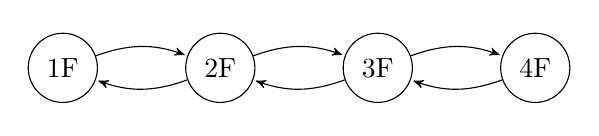
\begin{tikzpicture}[>=stealth',shorten >=1pt,auto,node distance=2cm]
  \node[state]  (q1)                {1F};
  \node[state]  (q2) [right of=q1]  {2F};
  \node[state]  (q3) [right of=q2]  {3F};
  \node[state]  (q4) [right of=q3]  {4F};

  \path[->]          (q1)  edge   [bend left=20]   node {} (q2);
  \path[->]          (q2)  edge   [bend left=20]   node {} (q1);

  \path[->]          (q2)  edge   [bend left=20]   node {} (q3);
  \path[->]          (q3)  edge   [bend left=20]   node {} (q2);

  \path[->]          (q3)  edge   [bend left=20]   node {} (q4);
  \path[->]          (q4)  edge   [bend left=20]   node {} (q3);

\end{tikzpicture}

\section{Liveness}

Consider the following elevator \textit{Spec}:
\begin{tla}
--------------------------- MODULE elevator ----------------------------
EXTENDS Integers
VARIABLES a
vars == <<a>>
TOP     == 4
BOTTOM  == 1
Init ==
    /\ a = BOTTOM
Up == 
    /\ a # TOP
    /\ a' = a + 1
Down == 
    /\ a # BOTTOM
    /\ a' = a - 1
Spec ==
  /\ Init
  /\ [][Up \/ Down]_a
=============================================================================
\end{tla}
\begin{tlatex}
\@x{}\moduleLeftDash\@xx{ {\MODULE} elevator}\moduleRightDash\@xx{}%
\@x{ {\EXTENDS} Integers}%
\@x{ {\VARIABLES} a}%
\@x{ vars \.{\defeq} {\langle} a {\rangle}}%
\@x{ TOP\@s{28.75} \.{\defeq} 4}%
\@x{ BOTTOM\@s{4.10} \.{\defeq} 1}%
\@x{ Init \.{\defeq}}%
\@x{\@s{16.4} \.{\land} a \.{=} BOTTOM}%
\@x{ Up \.{\defeq}}%
\@x{\@s{17.27} \.{\land} a \.{\neq} TOP}%
\@x{\@s{17.27} \.{\land} a \.{'} \.{=} a \.{+} 1}%
\@x{ Down \.{\defeq}}%
\@x{\@s{16.4} \.{\land} a \.{\neq} BOTTOM}%
\@x{\@s{16.4} \.{\land} a \.{'} \.{=} a \.{-} 1}%
\@x{ Spec \.{\defeq}}%
\@x{\@s{8.2} \.{\land}\@s{0.16} Init}%
\@x{\@s{8.2} \.{\land}\@s{0.16} {\Box} [ Up \.{\lor} Down ]_{ a}}%
\@x{}\bottombar\@xx{}%
\end{tlatex}

The building has a set of floors and the elevator can go either up or down. The
elevator keeps going up until it's the top floor, or keep going down until it's
the bottom floor. TLC will pass the \textit{Spec} as is.\newline

Let's introduce a liveness property. The elevator should always at least go 
to the second floor:\newline
\begin{tla}
Liveness == 
    /\ a = 1 ~> a = 2
\end{tla}
\begin{tlatex}
\@x{ Liveness \.{\defeq}}%
\@x{\@s{16.4} \.{\land} a \.{=} 1 \.{\leadsto} a \.{=} 2}%
\end{tlatex}
\newline

Running the \textit{Spec} against TLC will report a violation:

\begin{verbatim}
Error: Temporal properties were violated.
Error: The following behavior constitutes a counter-example:
State 1: <Initial predicate>
a = 1
State 2: Stuttering
\end{verbatim}

Since the \textit{Spec} permits \textit{suttering}, the state machine is allowed
to perpetually stay on 1F and \textit{never} go to 2F. This can be fixed by
introduce fairness description.

\section{Weak Fairness}

Weak fairness is defined as:\newline
\begin{equation} 
\Diamond\Box(ENABLED\langle A \rangle _v) \implies \Box\Diamond\langle A \rangle _v
\end{equation}
$ENABLED\langle A \rangle$ represents \textit{conditions required} for action A.
The above translates to: if conditions required for action A to occur is
\textit{eventually always} true, then action A will \textit{always eventually}
happen.\newline 

Without weak fairness defined, the elevator may \textit{stutter} at floor 1 and
never go to floor 2. Weak fairness states that if the conditions of an action is
\textit{eventually always} true (ie. elevator decides to stay on 1F but but
\textit{can} go up), the elevator \textit{always eventually} go up.\newline

\begin{tla}
Spec ==
  /\ Init
  /\ [][Down \/ Up]_a
  /\ WF_a(Down)
  /\ WF_a(Up)
\end{tla}
\begin{tlatex}
\@x{ Spec \.{\defeq}}%
\@x{\@s{8.2} \.{\land}\@s{0.16} Init}%
\@x{\@s{8.2} \.{\land}\@s{0.16} {\Box} [ Down \.{\lor} Up ]_{ a}}%
\@x{\@s{8.2} \.{\land}\@s{0.16} {\WF}_{ a} ( Down )}%
\@x{\@s{8.2} \.{\land}\@s{0.16} {\WF}_{ a} ( Up )}%
\end{tlatex}
\newline

Running the spec against TLC passes again. What if we want to verify the
elevator eventually always goes to the top, not just to 2F? Let's modify the
Liveness property again:\newline
\begin{tla}
Liveness == 
    /\ a = BOTTOM ~> a = TOP
\end{tla}
\begin{tlatex}
\@x{ Liveness \.{\defeq}}%
\@x{\@s{16.4} \.{\land} a \.{=} BOTTOM \.{\leadsto} a \.{=} TOP}%
\end{tlatex}
\newline

TLC now reports the following violation: 
\begin{verbatim}
Error: Temporal properties were violated.
Error: The following behavior constitutes a counter-example:
State 1: <Initial predicate>
a = 1
State 2: <Up line 10, col 5 to line 11, col 17 of module elevator>
a = 2
Back to state 1: <Down line 13, col 5 to line 14, col 17 of module elevator>
\end{verbatim}

TLC identified a case where the elevator is perpetually stuck going between 1F
and 2F, but never go to 3F. Weak fairness is no longer enough, because the the
elevator is not stuck on 2F repeatedly, but stuck going between 1F and 2F. This
is where we need strong fairness.

\section{Strong Fairness}

Strong fairness is defined as:\newline
\begin{equation} 
\Box\Diamond(ENABLED\langle A \rangle _v) \implies \Box\Diamond\langle A \rangle _v
\end{equation}
The difference between weak and strong fairness is the \textit{eventually
always} vs. \textit{always eventually}. \newline 

In weak fairness, once the state machine is stuck in a state forever, the state
machine always transition to a possible next state permitted by the spec (eg. if
the elevator is stuck on 1F but can go to 2F, it will). With strong fairness,
the elevator doesn't need to be stuck on 2F to go to 3F. If the elevator
\textit{always eventually} makes it to 2F, it \textit{eventually always} go to
3F.\newline 

Intuitively we are tempted to enable strong fairness like so: \newline
\begin{tla}
Spec ==
  /\ Init
  /\ [][Up \/ Down]_a
  /\ WF_a(Down)
  /\ SF_a(UP)
\end{tla}
\begin{tlatex}
\@x{ Spec \.{\defeq}}%
\@x{\@s{8.2} \.{\land}\@s{0.16} Init}%
\@x{\@s{8.2} \.{\land}\@s{0.16} {\Box} [ Up \.{\lor} Down ]_{ a}}%
\@x{\@s{8.2} \.{\land}\@s{0.16} {\WF}_{ a} ( Down )}%
\@x{\@s{8.2} \.{\land}\@s{0.16} {\SF}_{ a} ( UP )}%
\end{tlatex}
\newline 

However, TLC \textit{still} reports the same violation. What's going on?\newline

If we take a closer look at the enabling condition for \textit{Up}, it only
requires current floor to be not the \textit{top floor}. When the elevator is
stuck in a loop going Up and Down between 1F and 2F indefinitely, strong
fairness for Up is \textit{already satisfied}. What we really want is strong
fairness on \textit{Up} for \textit{every floor}, instead of \textit{any floor
except top floor}. So if elevator makes to 2F once, it will \textit{always
eventaully} go to 3F. If elevator makes to 3F once, it will \textit{always
eventaully} go to 4F, etc. The following is the change required:\newline

\begin{tla}
Spec ==
  /\ Init
  /\ [][Up \/ Down]_a
  /\ WF_a(Down)
  /\ \A f \in BOTTOM..TOP-1: 
    /\ WF_a(Up /\ f = a)
\end{tla}
\begin{tlatex}
\@x{ Spec \.{\defeq}}%
\@x{\@s{8.2} \.{\land}\@s{0.16} Init}%
\@x{\@s{8.2} \.{\land}\@s{0.16} {\Box} [ Up \.{\lor} Down ]_{ a}}%
\@x{\@s{8.2} \.{\land}\@s{0.16} {\WF}_{ a} ( Down )}%
 \@x{\@s{8.2} \.{\land}\@s{0.16} \A\, f \.{\in} BOTTOM \.{\dotdot} TOP \.{-} 1
 \.{:}}%
\@x{\@s{16.4} \.{\land} {\WF}_{ a} ( Up \.{\land} f \.{=} a )}%
\end{tlatex}
\newline

Once again with this change TLC will pass.

\chapter{TLA+ Abstraction Guideline}

\chapter{Reference}

\begin{thebibliography}{9}

\bibitem{}
Srikumar Subramanian
\textit{https://sriku.org/posts/fairness-in-tlaplus/}, 2015

\bibitem{}
% https://www.cds.caltech.edu/~murray/courses/afrl-sp12/L3_ltl-24Apr12.pdf
Richard M. Murray, Nok Wongpiromsarn
\textit{Linear Temporal Logic, Lecture 3}, 2012

\bibitem{backblaze}
\textit{https://www.backblaze.com/blog/cloud-storage-durability/}

\bibitem{raft}
\textit{https://raft.github.io/raft.pdf}

\bibitem{raft_tla}
\textit{https://github.com/ongardie/raft.tla}

\end{thebibliography}

\chapter{Nano}

TODO: add this to reference\newline
https://content.nano.org/whitepaper/Nano\_Whitepaper\_en.pdf

\section{Requirement}

\section{Spec}

\begin{tla}
Init ==
    /\ lastHash = NoHash
    /\ distributedLedger = [n \in Node |-> [h \in Hash |-> NoBlock]]
    /\ received = [n \in Node |-> {}]
\end{tla}
\begin{tlatex}
\@x{ Init \.{\defeq}}%
\@x{\@s{16.4} \.{\land} lastHash \.{=} NoHash}%
 \@x{\@s{16.4} \.{\land} distributedLedger \.{=} [ n \.{\in} Node \.{\mapsto}
 [ h \.{\in} Hash \.{\mapsto} NoBlock ] ]}%
\@x{\@s{16.4} \.{\land} received \.{=} [ n \.{\in} Node \.{\mapsto} \{ \} ]}%
\end{tlatex}

\begin{itemize}
    \item Every node is a ledger in this system, initialized to NoBlock
    \item Every node's received set is initialized to empty set
\end{itemize}

\begin{tla}
Next ==
    \/ \E account \in PrivateKey : CreateGenesisBlock(account)
    \/ \E node \in Node : CreateBlock(node)
    \/ \E node \in Node : ProcessBlock(node)
\end{tla}
\begin{tlatex}
\@x{ Next \.{\defeq}}%
 \@x{\@s{16.4} \.{\lor} \E\, account \.{\in} PrivateKey \.{:}
 CreateGenesisBlock ( account )}%
\@x{\@s{16.4} \.{\lor} \E\, node \.{\in} Node \.{:} CreateBlock ( node )}%
\@x{\@s{16.4} \.{\lor} \E\, node \.{\in} Node \.{:} ProcessBlock ( node )}%
\end{tlatex}
\newline

PrivateKey represents the identity of the account, create the genesis block for
every account. Let us look at how a genesis block is created:\newline

\begin{tla}
HashOf(block) ==
  IF \E hash \in Hash : hashFunction[hash] = block
  THEN CHOOSE hash \in Hash : hashFunction[hash] = block
  ELSE CHOOSE hash \in Hash : hashFunction[hash] = N!NoBlock

CalculateHashImpl(block, oldLastHash, newLastHash) ==
  LET hash == HashOf(block) IN
  /\ newLastHash = hash
  /\ hashFunction' = [hashFunction EXCEPT ![hash] = block]

CreateGenesisBlock(privateKey) ==
    LET
        publicKey == KeyPair[privateKey]
        genesisBlock ==
            [type   |-> "genesis",
            account |-> publicKey,
            balance |-> GenesisBalance]
    IN
    /\ ~GenesisBlockExists
    /\ CalculateHash(genesisBlock, lastHash, lastHash')
    /\ distributedLedger' =
        LET signedGenesisBlock ==
            [block |-> genesisBlock,
            signature |-> SignHash(lastHash', privateKey)]
        IN
        [n \in Node |->
            [distributedLedger[n] EXCEPT
                ![lastHash'] = signedGenesisBlock]]
    /\ UNCHANGED received
\end{tla}
\begin{tlatex}
\@x{ HashOf ( block ) \.{\defeq}}%
 \@x{\@s{8.2} {\IF} \E\, hash \.{\in} Hash \.{:} hashFunction [ hash ] \.{=}
 block}%
 \@x{\@s{8.2} \.{\THEN} {\CHOOSE} hash \.{\in} Hash \.{:} hashFunction [ hash
 ] \.{=} block}%
 \@x{\@s{8.2} \.{\ELSE} {\CHOOSE} hash \.{\in} Hash \.{:} hashFunction [ hash
 ] \.{=} N {\bang} NoBlock}%
\@pvspace{8.0pt}%
\@x{ CalculateHashImpl ( block ,\, oldLastHash ,\, newLastHash ) \.{\defeq}}%
\@x{\@s{8.2} \.{\LET} hash \.{\defeq} HashOf ( block ) \.{\IN}}%
\@x{\@s{8.2} \.{\land} newLastHash \.{=} hash}%
 \@x{\@s{8.2} \.{\land} hashFunction \.{'} \.{=} [ hashFunction {\EXCEPT}
 {\bang} [ hash ] \.{=} block ]}%
\@pvspace{8.0pt}%
\@x{ CreateGenesisBlock ( privateKey ) \.{\defeq}}%
\@x{\@s{16.4} \.{\LET}}%
\@x{\@s{32.8} publicKey \.{\defeq} KeyPair [ privateKey ]}%
\@x{\@s{32.8} genesisBlock \.{\defeq}}%
\@x{\@s{49.19} [ type\@s{12.75} \.{\mapsto}\@w{genesis} ,\,}%
\@x{\@s{49.19} account \.{\mapsto} publicKey ,\,}%
\@x{\@s{49.19} balance\@s{1.73} \.{\mapsto} GenesisBalance ]}%
\@x{\@s{16.4} \.{\IN}}%
\@x{\@s{16.4} \.{\land} {\lnot} GenesisBlockExists}%
 \@x{\@s{16.4} \.{\land} CalculateHash ( genesisBlock ,\, lastHash ,\,
 lastHash \.{'} )}%
\@x{\@s{16.4} \.{\land} distributedLedger \.{'} \.{=}}%
\@x{\@s{31.61} \.{\LET} signedGenesisBlock \.{\defeq}}%
\@x{\@s{52.01} [ block \.{\mapsto} genesisBlock ,\,}%
 \@x{\@s{52.01} signature \.{\mapsto} SignHash ( lastHash \.{'} ,\, privateKey
 ) ]}%
\@x{\@s{31.61} \.{\IN}}%
\@x{\@s{31.61} [ n \.{\in} Node \.{\mapsto}}%
\@x{\@s{44.87} [ distributedLedger [ n ] {\EXCEPT}}%
\@x{\@s{59.95} {\bang} [ lastHash \.{'} ] \.{=} signedGenesisBlock ] ]}%
\@x{\@s{16.4} \.{\land} {\UNCHANGED} received}%
\end{tlatex}
\newline

Every account maintains its own chain of blocks. The first block in the account
chain is the genesis block. The genesis block contains the type, account name,
and genesis balance. The genesis block is then hashed and signed.


% \chapter{Nano Blockchain}

TODO: add this to reference\newline
https://content.nano.org/whitepaper/Nano\_Whitepaper\_en.pdf


\end{document}
